% Created by tikzDevice version 0.12.4 on 2023-03-22 21:32:54
% !TEX encoding = UTF-8 Unicode
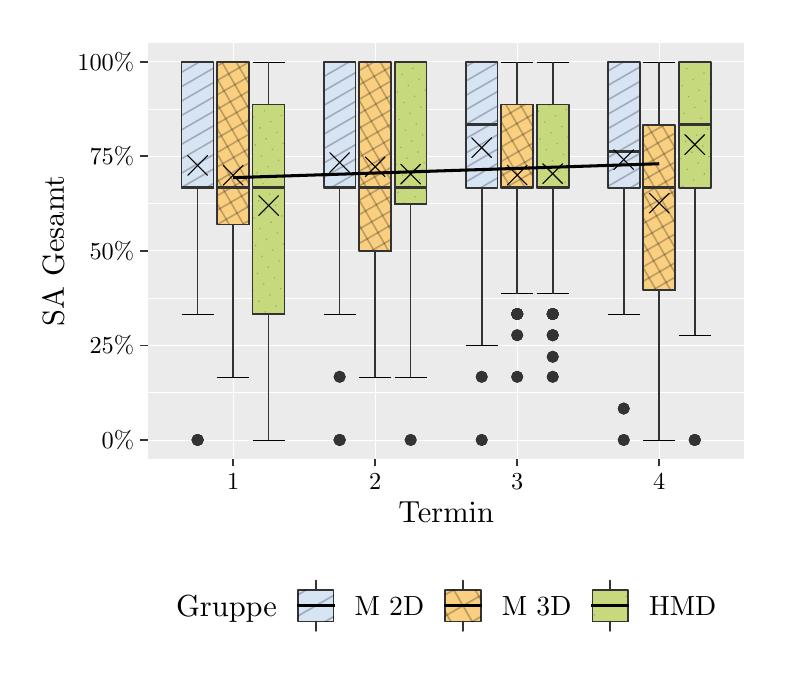
\begin{tikzpicture}[x=1pt,y=1pt]
\definecolor{fillColor}{RGB}{255,255,255}
\path[use as bounding box,fill=fillColor,fill opacity=0.00] (0,0) rectangle (264.51,231.26);
\begin{scope}
\path[clip] (  0.00,  0.00) rectangle (264.51,231.26);
\definecolor{drawColor}{RGB}{255,255,255}
\definecolor{fillColor}{RGB}{255,255,255}

\path[draw=drawColor,line width= 0.6pt,line join=round,line cap=round,fill=fillColor] (  0.00, -0.00) rectangle (264.51,231.26);
\end{scope}
\begin{scope}
\path[clip] ( 43.44, 75.45) rectangle (259.01,225.76);
\definecolor{fillColor}{gray}{0.92}

\path[fill=fillColor] ( 43.44, 75.45) rectangle (259.01,225.76);
\definecolor{drawColor}{RGB}{255,255,255}

\path[draw=drawColor,line width= 0.3pt,line join=round] ( 43.44, 99.36) --
	(259.01, 99.36);

\path[draw=drawColor,line width= 0.3pt,line join=round] ( 43.44,133.52) --
	(259.01,133.52);

\path[draw=drawColor,line width= 0.3pt,line join=round] ( 43.44,167.69) --
	(259.01,167.69);

\path[draw=drawColor,line width= 0.3pt,line join=round] ( 43.44,201.85) --
	(259.01,201.85);

\path[draw=drawColor,line width= 0.3pt,line join=round] ( 43.44, 82.28) --
	(259.01, 82.28);

\path[draw=drawColor,line width= 0.3pt,line join=round] ( 43.44,116.44) --
	(259.01,116.44);

\path[draw=drawColor,line width= 0.3pt,line join=round] ( 43.44,150.61) --
	(259.01,150.61);

\path[draw=drawColor,line width= 0.3pt,line join=round] ( 43.44,184.77) --
	(259.01,184.77);

\path[draw=drawColor,line width= 0.3pt,line join=round] ( 43.44,218.93) --
	(259.01,218.93);

\path[draw=drawColor,line width= 0.3pt,line join=round] ( 74.24, 75.45) --
	( 74.24,225.76);

\path[draw=drawColor,line width= 0.3pt,line join=round] (125.56, 75.45) --
	(125.56,225.76);

\path[draw=drawColor,line width= 0.3pt,line join=round] (176.89, 75.45) --
	(176.89,225.76);

\path[draw=drawColor,line width= 0.3pt,line join=round] (228.21, 75.45) --
	(228.21,225.76);
\definecolor{drawColor}{RGB}{0,0,0}

\path[draw=drawColor,line width= 0.2pt,line join=round] ( 55.63,218.93) --
	( 67.18,218.93);

\path[draw=drawColor,line width= 0.2pt,line join=round] ( 61.41,218.93) --
	( 61.41,127.79);

\path[draw=drawColor,line width= 0.2pt,line join=round] ( 55.63,127.79) --
	( 67.18,127.79);

\path[draw=drawColor,line width= 0.2pt,line join=round] ( 68.46,218.93) --
	( 80.01,218.93);

\path[draw=drawColor,line width= 0.2pt,line join=round] ( 74.24,218.93) --
	( 74.24,105.10);

\path[draw=drawColor,line width= 0.2pt,line join=round] ( 68.46,105.10) --
	( 80.01,105.10);

\path[draw=drawColor,line width= 0.2pt,line join=round] ( 81.30,218.93) --
	( 92.84,218.93);

\path[draw=drawColor,line width= 0.2pt,line join=round] ( 87.07,218.93) --
	( 87.07, 82.28);

\path[draw=drawColor,line width= 0.2pt,line join=round] ( 81.30, 82.28) --
	( 92.84, 82.28);

\path[draw=drawColor,line width= 0.2pt,line join=round] (106.96,218.93) --
	(118.51,218.93);

\path[draw=drawColor,line width= 0.2pt,line join=round] (112.73,218.93) --
	(112.73,127.79);

\path[draw=drawColor,line width= 0.2pt,line join=round] (106.96,127.79) --
	(118.51,127.79);

\path[draw=drawColor,line width= 0.2pt,line join=round] (119.79,218.93) --
	(131.34,218.93);

\path[draw=drawColor,line width= 0.2pt,line join=round] (125.56,218.93) --
	(125.56,105.10);

\path[draw=drawColor,line width= 0.2pt,line join=round] (119.79,105.10) --
	(131.34,105.10);

\path[draw=drawColor,line width= 0.2pt,line join=round] (132.62,218.93) --
	(144.17,218.93);

\path[draw=drawColor,line width= 0.2pt,line join=round] (138.39,218.93) --
	(138.39,105.10);

\path[draw=drawColor,line width= 0.2pt,line join=round] (132.62,105.10) --
	(144.17,105.10);

\path[draw=drawColor,line width= 0.2pt,line join=round] (158.28,218.93) --
	(169.83,218.93);

\path[draw=drawColor,line width= 0.2pt,line join=round] (164.06,218.93) --
	(164.06,116.44);

\path[draw=drawColor,line width= 0.2pt,line join=round] (158.28,116.44) --
	(169.83,116.44);

\path[draw=drawColor,line width= 0.2pt,line join=round] (171.11,218.93) --
	(182.66,218.93);

\path[draw=drawColor,line width= 0.2pt,line join=round] (176.89,218.93) --
	(176.89,135.16);

\path[draw=drawColor,line width= 0.2pt,line join=round] (171.11,135.16) --
	(182.66,135.16);

\path[draw=drawColor,line width= 0.2pt,line join=round] (183.95,218.93) --
	(195.49,218.93);

\path[draw=drawColor,line width= 0.2pt,line join=round] (189.72,218.93) --
	(189.72,135.16);

\path[draw=drawColor,line width= 0.2pt,line join=round] (183.95,135.16) --
	(195.49,135.16);

\path[draw=drawColor,line width= 0.2pt,line join=round] (209.61,218.93) --
	(221.16,218.93);

\path[draw=drawColor,line width= 0.2pt,line join=round] (215.38,218.93) --
	(215.38,127.79);

\path[draw=drawColor,line width= 0.2pt,line join=round] (209.61,127.79) --
	(221.16,127.79);

\path[draw=drawColor,line width= 0.2pt,line join=round] (222.44,218.93) --
	(233.99,218.93);

\path[draw=drawColor,line width= 0.2pt,line join=round] (228.21,218.93) --
	(228.21, 82.28);

\path[draw=drawColor,line width= 0.2pt,line join=round] (222.44, 82.28) --
	(233.99, 82.28);

\path[draw=drawColor,line width= 0.2pt,line join=round] (235.27,218.93) --
	(246.82,218.93);

\path[draw=drawColor,line width= 0.2pt,line join=round] (241.04,218.93) --
	(241.04,120.13);

\path[draw=drawColor,line width= 0.2pt,line join=round] (235.27,120.13) --
	(246.82,120.13);
\definecolor{drawColor}{gray}{0.20}
\definecolor{fillColor}{gray}{0.20}

\path[draw=drawColor,line width= 0.4pt,line join=round,line cap=round,fill=fillColor] ( 61.41, 82.28) circle (  1.96);

\path[draw=drawColor,line width= 0.4pt,line join=round,line cap=round,fill=fillColor] ( 61.41, 82.28) circle (  1.96);

\path[draw=drawColor,line width= 0.2pt,line join=round] ( 61.41,218.93) -- ( 61.41,218.93);

\path[draw=drawColor,line width= 0.2pt,line join=round] ( 61.41,173.43) -- ( 61.41,127.79);
\definecolor{fillColor}{RGB}{215,228,244}

\path[draw=drawColor,line width= 0.2pt,fill=fillColor] ( 55.63,218.93) --
	( 55.63,173.43) --
	( 67.18,173.43) --
	( 67.18,218.93) --
	( 55.63,218.93) --
	cycle;

\path[draw=drawColor,line width= 0.5pt] ( 55.63,173.43) -- ( 67.18,173.43);

\path[draw=drawColor,line width= 0.2pt,line join=round] ( 74.24,218.93) -- ( 74.24,218.93);

\path[draw=drawColor,line width= 0.2pt,line join=round] ( 74.24,160.17) -- ( 74.24,105.10);
\definecolor{fillColor}{RGB}{250,208,128}

\path[draw=drawColor,line width= 0.2pt,fill=fillColor] ( 68.46,218.93) --
	( 68.46,160.17) --
	( 80.01,160.17) --
	( 80.01,218.93) --
	( 68.46,218.93) --
	cycle;

\path[draw=drawColor,line width= 0.5pt] ( 68.46,173.43) -- ( 80.01,173.43);

\path[draw=drawColor,line width= 0.2pt,line join=round] ( 87.07,203.49) -- ( 87.07,218.93);

\path[draw=drawColor,line width= 0.2pt,line join=round] ( 87.07,127.79) -- ( 87.07, 82.28);
\definecolor{fillColor}{RGB}{199,217,125}

\path[draw=drawColor,line width= 0.2pt,fill=fillColor] ( 81.30,203.49) --
	( 81.30,127.79) --
	( 92.84,127.79) --
	( 92.84,203.49) --
	( 81.30,203.49) --
	cycle;

\path[draw=drawColor,line width= 0.5pt] ( 81.30,173.43) -- ( 92.84,173.43);
\definecolor{fillColor}{gray}{0.20}

\path[draw=drawColor,line width= 0.4pt,line join=round,line cap=round,fill=fillColor] (112.73, 82.28) circle (  1.96);

\path[draw=drawColor,line width= 0.4pt,line join=round,line cap=round,fill=fillColor] (112.73,105.10) circle (  1.96);

\path[draw=drawColor,line width= 0.4pt,line join=round,line cap=round,fill=fillColor] (112.73, 82.28) circle (  1.96);

\path[draw=drawColor,line width= 0.2pt,line join=round] (112.73,218.93) -- (112.73,218.93);

\path[draw=drawColor,line width= 0.2pt,line join=round] (112.73,173.43) -- (112.73,127.79);
\definecolor{fillColor}{RGB}{215,228,244}

\path[draw=drawColor,line width= 0.2pt,fill=fillColor] (106.96,218.93) --
	(106.96,173.43) --
	(118.51,173.43) --
	(118.51,218.93) --
	(106.96,218.93) --
	cycle;

\path[draw=drawColor,line width= 0.5pt] (106.96,173.43) -- (118.51,173.43);

\path[draw=drawColor,line width= 0.2pt,line join=round] (125.56,218.93) -- (125.56,218.93);

\path[draw=drawColor,line width= 0.2pt,line join=round] (125.56,150.61) -- (125.56,105.10);
\definecolor{fillColor}{RGB}{250,208,128}

\path[draw=drawColor,line width= 0.2pt,fill=fillColor] (119.79,218.93) --
	(119.79,150.61) --
	(131.34,150.61) --
	(131.34,218.93) --
	(119.79,218.93) --
	cycle;

\path[draw=drawColor,line width= 0.5pt] (119.79,173.43) -- (131.34,173.43);
\definecolor{fillColor}{gray}{0.20}

\path[draw=drawColor,line width= 0.4pt,line join=round,line cap=round,fill=fillColor] (138.39, 82.28) circle (  1.96);

\path[draw=drawColor,line width= 0.2pt,line join=round] (138.39,218.93) -- (138.39,218.93);

\path[draw=drawColor,line width= 0.2pt,line join=round] (138.39,167.58) -- (138.39,105.10);
\definecolor{fillColor}{RGB}{199,217,125}

\path[draw=drawColor,line width= 0.2pt,fill=fillColor] (132.62,218.93) --
	(132.62,167.58) --
	(144.17,167.58) --
	(144.17,218.93) --
	(132.62,218.93) --
	cycle;

\path[draw=drawColor,line width= 0.5pt] (132.62,173.43) -- (144.17,173.43);
\definecolor{fillColor}{gray}{0.20}

\path[draw=drawColor,line width= 0.4pt,line join=round,line cap=round,fill=fillColor] (164.06, 82.28) circle (  1.96);

\path[draw=drawColor,line width= 0.4pt,line join=round,line cap=round,fill=fillColor] (164.06,105.10) circle (  1.96);

\path[draw=drawColor,line width= 0.2pt,line join=round] (164.06,218.93) -- (164.06,218.93);

\path[draw=drawColor,line width= 0.2pt,line join=round] (164.06,173.43) -- (164.06,116.44);
\definecolor{fillColor}{RGB}{215,228,244}

\path[draw=drawColor,line width= 0.2pt,fill=fillColor] (158.28,218.93) --
	(158.28,173.43) --
	(169.83,173.43) --
	(169.83,218.93) --
	(158.28,218.93) --
	cycle;

\path[draw=drawColor,line width= 0.5pt] (158.28,196.11) -- (169.83,196.11);
\definecolor{fillColor}{gray}{0.20}

\path[draw=drawColor,line width= 0.4pt,line join=round,line cap=round,fill=fillColor] (176.89,127.79) circle (  1.96);

\path[draw=drawColor,line width= 0.4pt,line join=round,line cap=round,fill=fillColor] (176.89,127.79) circle (  1.96);

\path[draw=drawColor,line width= 0.4pt,line join=round,line cap=round,fill=fillColor] (176.89,127.79) circle (  1.96);

\path[draw=drawColor,line width= 0.4pt,line join=round,line cap=round,fill=fillColor] (176.89,127.79) circle (  1.96);

\path[draw=drawColor,line width= 0.4pt,line join=round,line cap=round,fill=fillColor] (176.89,120.13) circle (  1.96);

\path[draw=drawColor,line width= 0.4pt,line join=round,line cap=round,fill=fillColor] (176.89,105.10) circle (  1.96);

\path[draw=drawColor,line width= 0.4pt,line join=round,line cap=round,fill=fillColor] (176.89,127.79) circle (  1.96);

\path[draw=drawColor,line width= 0.2pt,line join=round] (176.89,203.49) -- (176.89,218.93);

\path[draw=drawColor,line width= 0.2pt,line join=round] (176.89,173.43) -- (176.89,135.16);
\definecolor{fillColor}{RGB}{250,208,128}

\path[draw=drawColor,line width= 0.2pt,fill=fillColor] (171.11,203.49) --
	(171.11,173.43) --
	(182.66,173.43) --
	(182.66,203.49) --
	(171.11,203.49) --
	cycle;

\path[draw=drawColor,line width= 0.5pt] (171.11,173.43) -- (182.66,173.43);
\definecolor{fillColor}{gray}{0.20}

\path[draw=drawColor,line width= 0.4pt,line join=round,line cap=round,fill=fillColor] (189.72,127.79) circle (  1.96);

\path[draw=drawColor,line width= 0.4pt,line join=round,line cap=round,fill=fillColor] (189.72,127.79) circle (  1.96);

\path[draw=drawColor,line width= 0.4pt,line join=round,line cap=round,fill=fillColor] (189.72,127.79) circle (  1.96);

\path[draw=drawColor,line width= 0.4pt,line join=round,line cap=round,fill=fillColor] (189.72,120.13) circle (  1.96);

\path[draw=drawColor,line width= 0.4pt,line join=round,line cap=round,fill=fillColor] (189.72,112.34) circle (  1.96);

\path[draw=drawColor,line width= 0.4pt,line join=round,line cap=round,fill=fillColor] (189.72,127.79) circle (  1.96);

\path[draw=drawColor,line width= 0.4pt,line join=round,line cap=round,fill=fillColor] (189.72,120.13) circle (  1.96);

\path[draw=drawColor,line width= 0.4pt,line join=round,line cap=round,fill=fillColor] (189.72,105.10) circle (  1.96);

\path[draw=drawColor,line width= 0.4pt,line join=round,line cap=round,fill=fillColor] (189.72,127.79) circle (  1.96);

\path[draw=drawColor,line width= 0.2pt,line join=round] (189.72,203.49) -- (189.72,218.93);

\path[draw=drawColor,line width= 0.2pt,line join=round] (189.72,173.43) -- (189.72,135.16);
\definecolor{fillColor}{RGB}{199,217,125}

\path[draw=drawColor,line width= 0.2pt,fill=fillColor] (183.95,203.49) --
	(183.95,173.43) --
	(195.49,173.43) --
	(195.49,203.49) --
	(183.95,203.49) --
	cycle;

\path[draw=drawColor,line width= 0.5pt] (183.95,173.43) -- (195.49,173.43);
\definecolor{fillColor}{gray}{0.20}

\path[draw=drawColor,line width= 0.4pt,line join=round,line cap=round,fill=fillColor] (215.38, 82.28) circle (  1.96);

\path[draw=drawColor,line width= 0.4pt,line join=round,line cap=round,fill=fillColor] (215.38, 93.62) circle (  1.96);

\path[draw=drawColor,line width= 0.2pt,line join=round] (215.38,218.93) -- (215.38,218.93);

\path[draw=drawColor,line width= 0.2pt,line join=round] (215.38,173.43) -- (215.38,127.79);
\definecolor{fillColor}{RGB}{215,228,244}

\path[draw=drawColor,line width= 0.2pt,fill=fillColor] (209.61,218.93) --
	(209.61,173.43) --
	(221.16,173.43) --
	(221.16,218.93) --
	(209.61,218.93) --
	cycle;

\path[draw=drawColor,line width= 0.5pt] (209.61,186.55) -- (221.16,186.55);

\path[draw=drawColor,line width= 0.2pt,line join=round] (228.21,196.11) -- (228.21,218.93);

\path[draw=drawColor,line width= 0.2pt,line join=round] (228.21,136.39) -- (228.21, 82.28);
\definecolor{fillColor}{RGB}{250,208,128}

\path[draw=drawColor,line width= 0.2pt,fill=fillColor] (222.44,196.11) --
	(222.44,136.39) --
	(233.99,136.39) --
	(233.99,196.11) --
	(222.44,196.11) --
	cycle;

\path[draw=drawColor,line width= 0.5pt] (222.44,173.43) -- (233.99,173.43);
\definecolor{fillColor}{gray}{0.20}

\path[draw=drawColor,line width= 0.4pt,line join=round,line cap=round,fill=fillColor] (241.04, 82.28) circle (  1.96);

\path[draw=drawColor,line width= 0.4pt,line join=round,line cap=round,fill=fillColor] (241.04, 82.28) circle (  1.96);

\path[draw=drawColor,line width= 0.2pt,line join=round] (241.04,218.93) -- (241.04,218.93);

\path[draw=drawColor,line width= 0.2pt,line join=round] (241.04,173.43) -- (241.04,120.13);
\definecolor{fillColor}{RGB}{199,217,125}

\path[draw=drawColor,line width= 0.2pt,fill=fillColor] (235.27,218.93) --
	(235.27,173.43) --
	(246.82,173.43) --
	(246.82,218.93) --
	(235.27,218.93) --
	cycle;

\path[draw=drawColor,line width= 0.5pt] (235.27,196.11) -- (246.82,196.11);
\definecolor{fillColor}{gray}{0.20}

\path[draw=drawColor,line width= 0.4pt,line join=round,line cap=round,fill=fillColor] ( 61.41, 82.28) circle (  1.96);

\path[draw=drawColor,line width= 0.4pt,line join=round,line cap=round,fill=fillColor] ( 61.41, 82.28) circle (  1.96);

\path[draw=drawColor,line width= 0.6pt,line join=round] ( 61.41,218.93) -- ( 61.41,218.93);

\path[draw=drawColor,line width= 0.6pt,line join=round] ( 61.41,173.43) -- ( 61.41,127.79);
\definecolor{fillColor}{RGB}{215,228,244}

\path[fill=fillColor] ( 55.63,218.93) --
	( 55.63,173.43) --
	( 67.18,173.43) --
	( 67.18,218.93) --
	( 55.63,218.93) --
	cycle;
\definecolor{drawColor}{RGB}{0,0,0}
\definecolor{fillColor}{RGB}{0,0,0}

\path[draw=drawColor,draw opacity=0.20,line width= 0.6pt,line join=round,line cap=rect,fill=fillColor,fill opacity=0.20] ( 67.18,175.01) --
	( 67.18,174.96) --
	( 64.53,173.43) --
	( 64.44,173.43) --
	( 67.18,175.01) --
	cycle;

\path[draw=drawColor,draw opacity=0.20,line width= 0.6pt,line join=round,line cap=rect,fill=fillColor,fill opacity=0.20] ( 67.18,180.22) --
	( 67.18,180.16) --
	( 55.63,173.50) --
	( 55.63,173.55) --
	( 67.18,180.22) --
	cycle;

\path[draw=drawColor,draw opacity=0.20,line width= 0.6pt,line join=round,line cap=rect,fill=fillColor,fill opacity=0.20] ( 67.18,185.42) --
	( 67.18,185.37) --
	( 55.63,178.70) --
	( 55.63,178.75) --
	( 67.18,185.42) --
	cycle;

\path[draw=drawColor,draw opacity=0.20,line width= 0.6pt,line join=round,line cap=rect,fill=fillColor,fill opacity=0.20] ( 67.18,190.63) --
	( 67.18,190.58) --
	( 55.63,183.91) --
	( 55.63,183.96) --
	( 67.18,190.63) --
	cycle;

\path[draw=drawColor,draw opacity=0.20,line width= 0.6pt,line join=round,line cap=rect,fill=fillColor,fill opacity=0.20] ( 67.18,195.84) --
	( 67.18,195.78) --
	( 55.63,189.12) --
	( 55.63,189.17) --
	( 67.18,195.84) --
	cycle;

\path[draw=drawColor,draw opacity=0.20,line width= 0.6pt,line join=round,line cap=rect,fill=fillColor,fill opacity=0.20] ( 67.18,201.04) --
	( 67.18,200.99) --
	( 55.63,194.32) --
	( 55.63,194.38) --
	( 67.18,201.04) --
	cycle;

\path[draw=drawColor,draw opacity=0.20,line width= 0.6pt,line join=round,line cap=rect,fill=fillColor,fill opacity=0.20] ( 67.18,206.25) --
	( 67.18,206.20) --
	( 55.63,199.53) --
	( 55.63,199.58) --
	( 67.18,206.25) --
	cycle;

\path[draw=drawColor,draw opacity=0.20,line width= 0.6pt,line join=round,line cap=rect,fill=fillColor,fill opacity=0.20] ( 67.18,211.46) --
	( 67.18,211.41) --
	( 55.63,204.74) --
	( 55.63,204.79) --
	( 67.18,211.46) --
	cycle;

\path[draw=drawColor,draw opacity=0.20,line width= 0.6pt,line join=round,line cap=rect,fill=fillColor,fill opacity=0.20] ( 67.18,216.66) --
	( 67.18,216.61) --
	( 55.63,209.95) --
	( 55.63,210.00) --
	( 67.18,216.66) --
	cycle;

\path[draw=drawColor,draw opacity=0.20,line width= 0.6pt,line join=round,line cap=rect,fill=fillColor,fill opacity=0.20] ( 62.09,218.93) --
	( 62.18,218.93) --
	( 55.63,215.15) --
	( 55.63,215.20) --
	( 62.09,218.93) --
	cycle;
\definecolor{drawColor}{gray}{0.20}

\path[draw=drawColor,line width= 0.6pt,line join=round,line cap=round] ( 55.63,218.93) --
	( 55.63,173.43) --
	( 67.18,173.43) --
	( 67.18,218.93) --
	( 55.63,218.93) --
	cycle;

\path[draw=drawColor,line width= 1.1pt,line join=round] ( 55.63,173.43) -- ( 67.18,173.43);
\definecolor{fillColor}{gray}{0.20}

\path[draw=drawColor,line width= 0.4pt,line join=round,line cap=round,fill=fillColor] (112.73, 82.28) circle (  1.96);

\path[draw=drawColor,line width= 0.4pt,line join=round,line cap=round,fill=fillColor] (112.73,105.10) circle (  1.96);

\path[draw=drawColor,line width= 0.4pt,line join=round,line cap=round,fill=fillColor] (112.73, 82.28) circle (  1.96);

\path[draw=drawColor,line width= 0.6pt,line join=round] (112.73,218.93) -- (112.73,218.93);

\path[draw=drawColor,line width= 0.6pt,line join=round] (112.73,173.43) -- (112.73,127.79);
\definecolor{fillColor}{RGB}{215,228,244}

\path[fill=fillColor] (106.96,218.93) --
	(106.96,173.43) --
	(118.51,173.43) --
	(118.51,218.93) --
	(106.96,218.93) --
	cycle;
\definecolor{drawColor}{RGB}{0,0,0}
\definecolor{fillColor}{RGB}{0,0,0}

\path[draw=drawColor,draw opacity=0.20,line width= 0.6pt,line join=round,line cap=rect,fill=fillColor,fill opacity=0.20] (118.51,178.61) --
	(118.51,178.55) --
	(109.63,173.43) --
	(109.54,173.43) --
	(118.51,178.61) --
	cycle;

\path[draw=drawColor,draw opacity=0.20,line width= 0.6pt,line join=round,line cap=rect,fill=fillColor,fill opacity=0.20] (118.51,183.81) --
	(118.51,183.76) --
	(106.96,177.09) --
	(106.96,177.14) --
	(118.51,183.81) --
	cycle;

\path[draw=drawColor,draw opacity=0.20,line width= 0.6pt,line join=round,line cap=rect,fill=fillColor,fill opacity=0.20] (118.51,189.02) --
	(118.51,188.97) --
	(106.96,182.30) --
	(106.96,182.35) --
	(118.51,189.02) --
	cycle;

\path[draw=drawColor,draw opacity=0.20,line width= 0.6pt,line join=round,line cap=rect,fill=fillColor,fill opacity=0.20] (118.51,194.23) --
	(118.51,194.17) --
	(106.96,187.51) --
	(106.96,187.56) --
	(118.51,194.23) --
	cycle;

\path[draw=drawColor,draw opacity=0.20,line width= 0.6pt,line join=round,line cap=rect,fill=fillColor,fill opacity=0.20] (118.51,199.43) --
	(118.51,199.38) --
	(106.96,192.71) --
	(106.96,192.77) --
	(118.51,199.43) --
	cycle;

\path[draw=drawColor,draw opacity=0.20,line width= 0.6pt,line join=round,line cap=rect,fill=fillColor,fill opacity=0.20] (118.51,204.64) --
	(118.51,204.59) --
	(106.96,197.92) --
	(106.96,197.97) --
	(118.51,204.64) --
	cycle;

\path[draw=drawColor,draw opacity=0.20,line width= 0.6pt,line join=round,line cap=rect,fill=fillColor,fill opacity=0.20] (118.51,209.85) --
	(118.51,209.80) --
	(106.96,203.13) --
	(106.96,203.18) --
	(118.51,209.85) --
	cycle;

\path[draw=drawColor,draw opacity=0.20,line width= 0.6pt,line join=round,line cap=rect,fill=fillColor,fill opacity=0.20] (118.51,215.05) --
	(118.51,215.00) --
	(106.96,208.34) --
	(106.96,208.39) --
	(118.51,215.05) --
	cycle;

\path[draw=drawColor,draw opacity=0.20,line width= 0.6pt,line join=round,line cap=rect,fill=fillColor,fill opacity=0.20] (116.20,218.93) --
	(116.29,218.93) --
	(106.96,213.54) --
	(106.96,213.59) --
	(116.20,218.93) --
	cycle;

\path[draw=drawColor,draw opacity=0.20,line width= 0.6pt,line join=round,line cap=rect,fill=fillColor,fill opacity=0.20] (107.18,218.93) --
	(107.27,218.93) --
	(106.96,218.75) --
	(106.96,218.80) --
	(107.18,218.93) --
	cycle;
\definecolor{drawColor}{gray}{0.20}

\path[draw=drawColor,line width= 0.6pt,line join=round,line cap=round] (106.96,218.93) --
	(106.96,173.43) --
	(118.51,173.43) --
	(118.51,218.93) --
	(106.96,218.93) --
	cycle;

\path[draw=drawColor,line width= 1.1pt,line join=round] (106.96,173.43) -- (118.51,173.43);
\definecolor{fillColor}{gray}{0.20}

\path[draw=drawColor,line width= 0.4pt,line join=round,line cap=round,fill=fillColor] (164.06, 82.28) circle (  1.96);

\path[draw=drawColor,line width= 0.4pt,line join=round,line cap=round,fill=fillColor] (164.06,105.10) circle (  1.96);

\path[draw=drawColor,line width= 0.6pt,line join=round] (164.06,218.93) -- (164.06,218.93);

\path[draw=drawColor,line width= 0.6pt,line join=round] (164.06,173.43) -- (164.06,116.44);
\definecolor{fillColor}{RGB}{215,228,244}

\path[fill=fillColor] (158.28,218.93) --
	(158.28,173.43) --
	(169.83,173.43) --
	(169.83,218.93) --
	(158.28,218.93) --
	cycle;
\definecolor{drawColor}{RGB}{0,0,0}
\definecolor{fillColor}{RGB}{0,0,0}

\path[draw=drawColor,draw opacity=0.20,line width= 0.6pt,line join=round,line cap=rect,fill=fillColor,fill opacity=0.20] (169.83,177.00) --
	(169.83,176.94) --
	(163.74,173.43) --
	(163.65,173.43) --
	(169.83,177.00) --
	cycle;

\path[draw=drawColor,draw opacity=0.20,line width= 0.6pt,line join=round,line cap=rect,fill=fillColor,fill opacity=0.20] (169.83,182.20) --
	(169.83,182.15) --
	(158.28,175.48) --
	(158.28,175.53) --
	(169.83,182.20) --
	cycle;

\path[draw=drawColor,draw opacity=0.20,line width= 0.6pt,line join=round,line cap=rect,fill=fillColor,fill opacity=0.20] (169.83,187.41) --
	(169.83,187.36) --
	(158.28,180.69) --
	(158.28,180.74) --
	(169.83,187.41) --
	cycle;

\path[draw=drawColor,draw opacity=0.20,line width= 0.6pt,line join=round,line cap=rect,fill=fillColor,fill opacity=0.20] (169.83,192.62) --
	(169.83,192.56) --
	(158.28,185.90) --
	(158.28,185.95) --
	(169.83,192.62) --
	cycle;

\path[draw=drawColor,draw opacity=0.20,line width= 0.6pt,line join=round,line cap=rect,fill=fillColor,fill opacity=0.20] (169.83,197.82) --
	(169.83,197.77) --
	(158.28,191.10) --
	(158.28,191.16) --
	(169.83,197.82) --
	cycle;

\path[draw=drawColor,draw opacity=0.20,line width= 0.6pt,line join=round,line cap=rect,fill=fillColor,fill opacity=0.20] (169.83,203.03) --
	(169.83,202.98) --
	(158.28,196.31) --
	(158.28,196.36) --
	(169.83,203.03) --
	cycle;

\path[draw=drawColor,draw opacity=0.20,line width= 0.6pt,line join=round,line cap=rect,fill=fillColor,fill opacity=0.20] (169.83,208.24) --
	(169.83,208.19) --
	(158.28,201.52) --
	(158.28,201.57) --
	(169.83,208.24) --
	cycle;

\path[draw=drawColor,draw opacity=0.20,line width= 0.6pt,line join=round,line cap=rect,fill=fillColor,fill opacity=0.20] (169.83,213.44) --
	(169.83,213.39) --
	(158.28,206.73) --
	(158.28,206.78) --
	(169.83,213.44) --
	cycle;

\path[draw=drawColor,draw opacity=0.20,line width= 0.6pt,line join=round,line cap=rect,fill=fillColor,fill opacity=0.20] (169.83,218.65) --
	(169.83,218.60) --
	(158.28,211.93) --
	(158.28,211.98) --
	(169.83,218.65) --
	cycle;

\path[draw=drawColor,draw opacity=0.20,line width= 0.6pt,line join=round,line cap=rect,fill=fillColor,fill opacity=0.20] (161.30,218.93) --
	(161.39,218.93) --
	(158.28,217.14) --
	(158.28,217.19) --
	(161.30,218.93) --
	cycle;
\definecolor{drawColor}{gray}{0.20}

\path[draw=drawColor,line width= 0.6pt,line join=round,line cap=round] (158.28,218.93) --
	(158.28,173.43) --
	(169.83,173.43) --
	(169.83,218.93) --
	(158.28,218.93) --
	cycle;

\path[draw=drawColor,line width= 1.1pt,line join=round] (158.28,196.11) -- (169.83,196.11);
\definecolor{fillColor}{gray}{0.20}

\path[draw=drawColor,line width= 0.4pt,line join=round,line cap=round,fill=fillColor] (215.38, 82.28) circle (  1.96);

\path[draw=drawColor,line width= 0.4pt,line join=round,line cap=round,fill=fillColor] (215.38, 93.62) circle (  1.96);

\path[draw=drawColor,line width= 0.6pt,line join=round] (215.38,218.93) -- (215.38,218.93);

\path[draw=drawColor,line width= 0.6pt,line join=round] (215.38,173.43) -- (215.38,127.79);
\definecolor{fillColor}{RGB}{215,228,244}

\path[fill=fillColor] (209.61,218.93) --
	(209.61,173.43) --
	(221.16,173.43) --
	(221.16,218.93) --
	(209.61,218.93) --
	cycle;
\definecolor{drawColor}{RGB}{0,0,0}
\definecolor{fillColor}{RGB}{0,0,0}

\path[draw=drawColor,draw opacity=0.20,line width= 0.6pt,line join=round,line cap=rect,fill=fillColor,fill opacity=0.20] (221.16,175.39) --
	(221.16,175.33) --
	(217.85,173.43) --
	(217.76,173.43) --
	(221.16,175.39) --
	cycle;

\path[draw=drawColor,draw opacity=0.20,line width= 0.6pt,line join=round,line cap=rect,fill=fillColor,fill opacity=0.20] (221.16,180.59) --
	(221.16,180.54) --
	(209.61,173.87) --
	(209.61,173.92) --
	(221.16,180.59) --
	cycle;

\path[draw=drawColor,draw opacity=0.20,line width= 0.6pt,line join=round,line cap=rect,fill=fillColor,fill opacity=0.20] (221.16,185.80) --
	(221.16,185.75) --
	(209.61,179.08) --
	(209.61,179.13) --
	(221.16,185.80) --
	cycle;

\path[draw=drawColor,draw opacity=0.20,line width= 0.6pt,line join=round,line cap=rect,fill=fillColor,fill opacity=0.20] (221.16,191.01) --
	(221.16,190.95) --
	(209.61,184.29) --
	(209.61,184.34) --
	(221.16,191.01) --
	cycle;

\path[draw=drawColor,draw opacity=0.20,line width= 0.6pt,line join=round,line cap=rect,fill=fillColor,fill opacity=0.20] (221.16,196.21) --
	(221.16,196.16) --
	(209.61,189.49) --
	(209.61,189.55) --
	(221.16,196.21) --
	cycle;

\path[draw=drawColor,draw opacity=0.20,line width= 0.6pt,line join=round,line cap=rect,fill=fillColor,fill opacity=0.20] (221.16,201.42) --
	(221.16,201.37) --
	(209.61,194.70) --
	(209.61,194.75) --
	(221.16,201.42) --
	cycle;

\path[draw=drawColor,draw opacity=0.20,line width= 0.6pt,line join=round,line cap=rect,fill=fillColor,fill opacity=0.20] (221.16,206.63) --
	(221.16,206.58) --
	(209.61,199.91) --
	(209.61,199.96) --
	(221.16,206.63) --
	cycle;

\path[draw=drawColor,draw opacity=0.20,line width= 0.6pt,line join=round,line cap=rect,fill=fillColor,fill opacity=0.20] (221.16,211.83) --
	(221.16,211.78) --
	(209.61,205.12) --
	(209.61,205.17) --
	(221.16,211.83) --
	cycle;

\path[draw=drawColor,draw opacity=0.20,line width= 0.6pt,line join=round,line cap=rect,fill=fillColor,fill opacity=0.20] (221.16,217.04) --
	(221.16,216.99) --
	(209.61,210.32) --
	(209.61,210.37) --
	(221.16,217.04) --
	cycle;

\path[draw=drawColor,draw opacity=0.20,line width= 0.6pt,line join=round,line cap=rect,fill=fillColor,fill opacity=0.20] (215.41,218.93) --
	(215.50,218.93) --
	(209.61,215.53) --
	(209.61,215.58) --
	(215.41,218.93) --
	cycle;
\definecolor{drawColor}{gray}{0.20}

\path[draw=drawColor,line width= 0.6pt,line join=round,line cap=round] (209.61,218.93) --
	(209.61,173.43) --
	(221.16,173.43) --
	(221.16,218.93) --
	(209.61,218.93) --
	cycle;

\path[draw=drawColor,line width= 1.1pt,line join=round] (209.61,186.55) -- (221.16,186.55);

\path[draw=drawColor,line width= 0.6pt,line join=round] ( 74.24,218.93) -- ( 74.24,218.93);

\path[draw=drawColor,line width= 0.6pt,line join=round] ( 74.24,160.17) -- ( 74.24,105.10);
\definecolor{fillColor}{RGB}{250,208,128}

\path[fill=fillColor] ( 68.46,218.93) --
	( 68.46,160.17) --
	( 80.01,160.17) --
	( 80.01,218.93) --
	( 68.46,218.93) --
	cycle;
\definecolor{drawColor}{RGB}{0,0,0}
\definecolor{fillColor}{RGB}{0,0,0}

\path[draw=drawColor,draw opacity=0.20,line width= 0.6pt,line join=round,line cap=rect,fill=fillColor,fill opacity=0.20] ( 80.01,161.59) --
	( 80.01,161.54) --
	( 77.65,160.17) --
	( 77.56,160.17) --
	( 80.01,161.59) --
	cycle;

\path[draw=drawColor,draw opacity=0.20,line width= 0.6pt,line join=round,line cap=rect,fill=fillColor,fill opacity=0.20] ( 80.01,166.79) --
	( 80.01,166.74) --
	( 68.63,160.17) --
	( 68.54,160.17) --
	( 80.01,166.79) --
	cycle;

\path[draw=drawColor,draw opacity=0.20,line width= 0.6pt,line join=round,line cap=rect,fill=fillColor,fill opacity=0.20] ( 80.01,172.00) --
	( 80.01,171.95) --
	( 68.46,165.28) --
	( 68.46,165.33) --
	( 80.01,172.00) --
	cycle;

\path[draw=drawColor,draw opacity=0.20,line width= 0.6pt,line join=round,line cap=rect,fill=fillColor,fill opacity=0.20] ( 80.01,177.21) --
	( 80.01,177.16) --
	( 68.46,170.49) --
	( 68.46,170.54) --
	( 80.01,177.21) --
	cycle;

\path[draw=drawColor,draw opacity=0.20,line width= 0.6pt,line join=round,line cap=rect,fill=fillColor,fill opacity=0.20] ( 80.01,182.42) --
	( 80.01,182.36) --
	( 68.46,175.70) --
	( 68.46,175.75) --
	( 80.01,182.42) --
	cycle;

\path[draw=drawColor,draw opacity=0.20,line width= 0.6pt,line join=round,line cap=rect,fill=fillColor,fill opacity=0.20] ( 80.01,187.62) --
	( 80.01,187.57) --
	( 68.46,180.90) --
	( 68.46,180.96) --
	( 80.01,187.62) --
	cycle;

\path[draw=drawColor,draw opacity=0.20,line width= 0.6pt,line join=round,line cap=rect,fill=fillColor,fill opacity=0.20] ( 80.01,192.83) --
	( 80.01,192.78) --
	( 68.46,186.11) --
	( 68.46,186.16) --
	( 80.01,192.83) --
	cycle;

\path[draw=drawColor,draw opacity=0.20,line width= 0.6pt,line join=round,line cap=rect,fill=fillColor,fill opacity=0.20] ( 80.01,198.04) --
	( 80.01,197.99) --
	( 68.46,191.32) --
	( 68.46,191.37) --
	( 80.01,198.04) --
	cycle;

\path[draw=drawColor,draw opacity=0.20,line width= 0.6pt,line join=round,line cap=rect,fill=fillColor,fill opacity=0.20] ( 80.01,203.24) --
	( 80.01,203.19) --
	( 68.46,196.53) --
	( 68.46,196.58) --
	( 80.01,203.24) --
	cycle;

\path[draw=drawColor,draw opacity=0.20,line width= 0.6pt,line join=round,line cap=rect,fill=fillColor,fill opacity=0.20] ( 80.01,208.45) --
	( 80.01,208.40) --
	( 68.46,201.73) --
	( 68.46,201.78) --
	( 80.01,208.45) --
	cycle;

\path[draw=drawColor,draw opacity=0.20,line width= 0.6pt,line join=round,line cap=rect,fill=fillColor,fill opacity=0.20] ( 80.01,213.66) --
	( 80.01,213.61) --
	( 68.46,206.94) --
	( 68.46,206.99) --
	( 80.01,213.66) --
	cycle;

\path[draw=drawColor,draw opacity=0.20,line width= 0.6pt,line join=round,line cap=rect,fill=fillColor,fill opacity=0.20] ( 80.01,218.87) --
	( 80.01,218.81) --
	( 68.46,212.15) --
	( 68.46,212.20) --
	( 80.01,218.87) --
	cycle;

\path[draw=drawColor,draw opacity=0.20,line width= 0.6pt,line join=round,line cap=rect,fill=fillColor,fill opacity=0.20] ( 71.11,218.93) --
	( 71.20,218.93) --
	( 68.46,217.35) --
	( 68.46,217.41) --
	( 71.11,218.93) --
	cycle;

\path[draw=drawColor,draw opacity=0.20,line width= 0.6pt,line join=round,line cap=rect,fill=fillColor,fill opacity=0.20] ( 72.83,160.17) --
	( 72.78,160.17) --
	( 68.46,167.64) --
	( 68.46,167.73) --
	( 72.83,160.17) --
	cycle;

\path[draw=drawColor,draw opacity=0.20,line width= 0.6pt,line join=round,line cap=rect,fill=fillColor,fill opacity=0.20] ( 78.04,160.17) --
	( 77.98,160.17) --
	( 68.46,176.66) --
	( 68.46,176.75) --
	( 78.04,160.17) --
	cycle;

\path[draw=drawColor,draw opacity=0.20,line width= 0.6pt,line join=round,line cap=rect,fill=fillColor,fill opacity=0.20] ( 80.01,165.77) --
	( 80.01,165.68) --
	( 68.46,185.68) --
	( 68.46,185.77) --
	( 80.01,165.77) --
	cycle;

\path[draw=drawColor,draw opacity=0.20,line width= 0.6pt,line join=round,line cap=rect,fill=fillColor,fill opacity=0.20] ( 80.01,174.79) --
	( 80.01,174.70) --
	( 68.46,194.70) --
	( 68.46,194.79) --
	( 80.01,174.79) --
	cycle;

\path[draw=drawColor,draw opacity=0.20,line width= 0.6pt,line join=round,line cap=rect,fill=fillColor,fill opacity=0.20] ( 80.01,183.81) --
	( 80.01,183.72) --
	( 68.46,203.72) --
	( 68.46,203.81) --
	( 80.01,183.81) --
	cycle;

\path[draw=drawColor,draw opacity=0.20,line width= 0.6pt,line join=round,line cap=rect,fill=fillColor,fill opacity=0.20] ( 80.01,192.83) --
	( 80.01,192.74) --
	( 68.46,212.74) --
	( 68.46,212.83) --
	( 80.01,192.83) --
	cycle;

\path[draw=drawColor,draw opacity=0.20,line width= 0.6pt,line join=round,line cap=rect,fill=fillColor,fill opacity=0.20] ( 80.01,201.84) --
	( 80.01,201.75) --
	( 70.09,218.93) --
	( 70.15,218.93) --
	( 80.01,201.84) --
	cycle;

\path[draw=drawColor,draw opacity=0.20,line width= 0.6pt,line join=round,line cap=rect,fill=fillColor,fill opacity=0.20] ( 80.01,210.86) --
	( 80.01,210.77) --
	( 75.30,218.93) --
	( 75.35,218.93) --
	( 80.01,210.86) --
	cycle;
\definecolor{drawColor}{gray}{0.20}

\path[draw=drawColor,line width= 0.6pt,line join=round,line cap=round] ( 68.46,218.93) --
	( 68.46,160.17) --
	( 80.01,160.17) --
	( 80.01,218.93) --
	( 68.46,218.93) --
	cycle;

\path[draw=drawColor,line width= 1.1pt,line join=round] ( 68.46,173.43) -- ( 80.01,173.43);

\path[draw=drawColor,line width= 0.6pt,line join=round] (125.56,218.93) -- (125.56,218.93);

\path[draw=drawColor,line width= 0.6pt,line join=round] (125.56,150.61) -- (125.56,105.10);
\definecolor{fillColor}{RGB}{250,208,128}

\path[fill=fillColor] (119.79,218.93) --
	(119.79,150.61) --
	(131.34,150.61) --
	(131.34,218.93) --
	(119.79,218.93) --
	cycle;
\definecolor{drawColor}{RGB}{0,0,0}
\definecolor{fillColor}{RGB}{0,0,0}

\path[draw=drawColor,draw opacity=0.20,line width= 0.6pt,line join=round,line cap=rect,fill=fillColor,fill opacity=0.20] (131.34,154.77) --
	(131.34,154.72) --
	(124.21,150.61) --
	(124.12,150.61) --
	(131.34,154.77) --
	cycle;

\path[draw=drawColor,draw opacity=0.20,line width= 0.6pt,line join=round,line cap=rect,fill=fillColor,fill opacity=0.20] (131.34,159.98) --
	(131.34,159.93) --
	(119.79,153.26) --
	(119.79,153.31) --
	(131.34,159.98) --
	cycle;

\path[draw=drawColor,draw opacity=0.20,line width= 0.6pt,line join=round,line cap=rect,fill=fillColor,fill opacity=0.20] (131.34,165.18) --
	(131.34,165.13) --
	(119.79,158.47) --
	(119.79,158.52) --
	(131.34,165.18) --
	cycle;

\path[draw=drawColor,draw opacity=0.20,line width= 0.6pt,line join=round,line cap=rect,fill=fillColor,fill opacity=0.20] (131.34,170.39) --
	(131.34,170.34) --
	(119.79,163.67) --
	(119.79,163.72) --
	(131.34,170.39) --
	cycle;

\path[draw=drawColor,draw opacity=0.20,line width= 0.6pt,line join=round,line cap=rect,fill=fillColor,fill opacity=0.20] (131.34,175.60) --
	(131.34,175.55) --
	(119.79,168.88) --
	(119.79,168.93) --
	(131.34,175.60) --
	cycle;

\path[draw=drawColor,draw opacity=0.20,line width= 0.6pt,line join=round,line cap=rect,fill=fillColor,fill opacity=0.20] (131.34,180.81) --
	(131.34,180.75) --
	(119.79,174.09) --
	(119.79,174.14) --
	(131.34,180.81) --
	cycle;

\path[draw=drawColor,draw opacity=0.20,line width= 0.6pt,line join=round,line cap=rect,fill=fillColor,fill opacity=0.20] (131.34,186.01) --
	(131.34,185.96) --
	(119.79,179.29) --
	(119.79,179.35) --
	(131.34,186.01) --
	cycle;

\path[draw=drawColor,draw opacity=0.20,line width= 0.6pt,line join=round,line cap=rect,fill=fillColor,fill opacity=0.20] (131.34,191.22) --
	(131.34,191.17) --
	(119.79,184.50) --
	(119.79,184.55) --
	(131.34,191.22) --
	cycle;

\path[draw=drawColor,draw opacity=0.20,line width= 0.6pt,line join=round,line cap=rect,fill=fillColor,fill opacity=0.20] (131.34,196.43) --
	(131.34,196.38) --
	(119.79,189.71) --
	(119.79,189.76) --
	(131.34,196.43) --
	cycle;

\path[draw=drawColor,draw opacity=0.20,line width= 0.6pt,line join=round,line cap=rect,fill=fillColor,fill opacity=0.20] (131.34,201.63) --
	(131.34,201.58) --
	(119.79,194.92) --
	(119.79,194.97) --
	(131.34,201.63) --
	cycle;

\path[draw=drawColor,draw opacity=0.20,line width= 0.6pt,line join=round,line cap=rect,fill=fillColor,fill opacity=0.20] (131.34,206.84) --
	(131.34,206.79) --
	(119.79,200.12) --
	(119.79,200.17) --
	(131.34,206.84) --
	cycle;

\path[draw=drawColor,draw opacity=0.20,line width= 0.6pt,line join=round,line cap=rect,fill=fillColor,fill opacity=0.20] (131.34,212.05) --
	(131.34,212.00) --
	(119.79,205.33) --
	(119.79,205.38) --
	(131.34,212.05) --
	cycle;

\path[draw=drawColor,draw opacity=0.20,line width= 0.6pt,line join=round,line cap=rect,fill=fillColor,fill opacity=0.20] (131.34,217.26) --
	(131.34,217.20) --
	(119.79,210.54) --
	(119.79,210.59) --
	(131.34,217.26) --
	cycle;

\path[draw=drawColor,draw opacity=0.20,line width= 0.6pt,line join=round,line cap=rect,fill=fillColor,fill opacity=0.20] (125.22,218.93) --
	(125.31,218.93) --
	(119.79,215.74) --
	(119.79,215.80) --
	(125.22,218.93) --
	cycle;

\path[draw=drawColor,draw opacity=0.20,line width= 0.6pt,line join=round,line cap=rect,fill=fillColor,fill opacity=0.20] (120.01,150.61) --
	(119.96,150.61) --
	(119.79,150.90) --
	(119.79,150.99) --
	(120.01,150.61) --
	cycle;

\path[draw=drawColor,draw opacity=0.20,line width= 0.6pt,line join=round,line cap=rect,fill=fillColor,fill opacity=0.20] (125.22,150.61) --
	(125.16,150.61) --
	(119.79,159.92) --
	(119.79,160.01) --
	(125.22,150.61) --
	cycle;

\path[draw=drawColor,draw opacity=0.20,line width= 0.6pt,line join=round,line cap=rect,fill=fillColor,fill opacity=0.20] (130.42,150.61) --
	(130.37,150.61) --
	(119.79,168.93) --
	(119.79,169.03) --
	(130.42,150.61) --
	cycle;

\path[draw=drawColor,draw opacity=0.20,line width= 0.6pt,line join=round,line cap=rect,fill=fillColor,fill opacity=0.20] (131.34,158.04) --
	(131.34,157.95) --
	(119.79,177.95) --
	(119.79,178.04) --
	(131.34,158.04) --
	cycle;

\path[draw=drawColor,draw opacity=0.20,line width= 0.6pt,line join=round,line cap=rect,fill=fillColor,fill opacity=0.20] (131.34,167.06) --
	(131.34,166.97) --
	(119.79,186.97) --
	(119.79,187.06) --
	(131.34,167.06) --
	cycle;

\path[draw=drawColor,draw opacity=0.20,line width= 0.6pt,line join=round,line cap=rect,fill=fillColor,fill opacity=0.20] (131.34,176.08) --
	(131.34,175.99) --
	(119.79,195.99) --
	(119.79,196.08) --
	(131.34,176.08) --
	cycle;

\path[draw=drawColor,draw opacity=0.20,line width= 0.6pt,line join=round,line cap=rect,fill=fillColor,fill opacity=0.20] (131.34,185.10) --
	(131.34,185.01) --
	(119.79,205.01) --
	(119.79,205.10) --
	(131.34,185.10) --
	cycle;

\path[draw=drawColor,draw opacity=0.20,line width= 0.6pt,line join=round,line cap=rect,fill=fillColor,fill opacity=0.20] (131.34,194.12) --
	(131.34,194.03) --
	(119.79,214.03) --
	(119.79,214.12) --
	(131.34,194.12) --
	cycle;

\path[draw=drawColor,draw opacity=0.20,line width= 0.6pt,line join=round,line cap=rect,fill=fillColor,fill opacity=0.20] (131.34,203.14) --
	(131.34,203.05) --
	(122.17,218.93) --
	(122.22,218.93) --
	(131.34,203.14) --
	cycle;

\path[draw=drawColor,draw opacity=0.20,line width= 0.6pt,line join=round,line cap=rect,fill=fillColor,fill opacity=0.20] (131.34,212.16) --
	(131.34,212.07) --
	(127.37,218.93) --
	(127.43,218.93) --
	(131.34,212.16) --
	cycle;
\definecolor{drawColor}{gray}{0.20}

\path[draw=drawColor,line width= 0.6pt,line join=round,line cap=round] (119.79,218.93) --
	(119.79,150.61) --
	(131.34,150.61) --
	(131.34,218.93) --
	(119.79,218.93) --
	cycle;

\path[draw=drawColor,line width= 1.1pt,line join=round] (119.79,173.43) -- (131.34,173.43);
\definecolor{fillColor}{gray}{0.20}

\path[draw=drawColor,line width= 0.4pt,line join=round,line cap=round,fill=fillColor] (176.89,127.79) circle (  1.96);

\path[draw=drawColor,line width= 0.4pt,line join=round,line cap=round,fill=fillColor] (176.89,127.79) circle (  1.96);

\path[draw=drawColor,line width= 0.4pt,line join=round,line cap=round,fill=fillColor] (176.89,127.79) circle (  1.96);

\path[draw=drawColor,line width= 0.4pt,line join=round,line cap=round,fill=fillColor] (176.89,127.79) circle (  1.96);

\path[draw=drawColor,line width= 0.4pt,line join=round,line cap=round,fill=fillColor] (176.89,120.13) circle (  1.96);

\path[draw=drawColor,line width= 0.4pt,line join=round,line cap=round,fill=fillColor] (176.89,105.10) circle (  1.96);

\path[draw=drawColor,line width= 0.4pt,line join=round,line cap=round,fill=fillColor] (176.89,127.79) circle (  1.96);

\path[draw=drawColor,line width= 0.6pt,line join=round] (176.89,203.49) -- (176.89,218.93);

\path[draw=drawColor,line width= 0.6pt,line join=round] (176.89,173.43) -- (176.89,135.16);
\definecolor{fillColor}{RGB}{250,208,128}

\path[fill=fillColor] (171.11,203.49) --
	(171.11,173.43) --
	(182.66,173.43) --
	(182.66,203.49) --
	(171.11,203.49) --
	cycle;
\definecolor{drawColor}{RGB}{0,0,0}
\definecolor{fillColor}{RGB}{0,0,0}

\path[draw=drawColor,draw opacity=0.20,line width= 0.6pt,line join=round,line cap=rect,fill=fillColor,fill opacity=0.20] (182.66,173.99) --
	(182.66,173.94) --
	(181.78,173.43) --
	(181.69,173.43) --
	(182.66,173.99) --
	cycle;

\path[draw=drawColor,draw opacity=0.20,line width= 0.6pt,line join=round,line cap=rect,fill=fillColor,fill opacity=0.20] (182.66,179.20) --
	(182.66,179.14) --
	(172.76,173.43) --
	(172.67,173.43) --
	(182.66,179.20) --
	cycle;

\path[draw=drawColor,draw opacity=0.20,line width= 0.6pt,line join=round,line cap=rect,fill=fillColor,fill opacity=0.20] (182.66,184.40) --
	(182.66,184.35) --
	(171.11,177.68) --
	(171.11,177.74) --
	(182.66,184.40) --
	cycle;

\path[draw=drawColor,draw opacity=0.20,line width= 0.6pt,line join=round,line cap=rect,fill=fillColor,fill opacity=0.20] (182.66,189.61) --
	(182.66,189.56) --
	(171.11,182.89) --
	(171.11,182.94) --
	(182.66,189.61) --
	cycle;

\path[draw=drawColor,draw opacity=0.20,line width= 0.6pt,line join=round,line cap=rect,fill=fillColor,fill opacity=0.20] (182.66,194.82) --
	(182.66,194.77) --
	(171.11,188.10) --
	(171.11,188.15) --
	(182.66,194.82) --
	cycle;

\path[draw=drawColor,draw opacity=0.20,line width= 0.6pt,line join=round,line cap=rect,fill=fillColor,fill opacity=0.20] (182.66,200.02) --
	(182.66,199.97) --
	(171.11,193.31) --
	(171.11,193.36) --
	(182.66,200.02) --
	cycle;

\path[draw=drawColor,draw opacity=0.20,line width= 0.6pt,line join=round,line cap=rect,fill=fillColor,fill opacity=0.20] (179.65,203.49) --
	(179.74,203.49) --
	(171.11,198.51) --
	(171.11,198.56) --
	(179.65,203.49) --
	cycle;

\path[draw=drawColor,draw opacity=0.20,line width= 0.6pt,line join=round,line cap=rect,fill=fillColor,fill opacity=0.20] (174.53,173.43) --
	(174.47,173.43) --
	(171.11,179.25) --
	(171.11,179.34) --
	(174.53,173.43) --
	cycle;

\path[draw=drawColor,draw opacity=0.20,line width= 0.6pt,line join=round,line cap=rect,fill=fillColor,fill opacity=0.20] (179.73,173.43) --
	(179.68,173.43) --
	(171.11,188.26) --
	(171.11,188.35) --
	(179.73,173.43) --
	cycle;

\path[draw=drawColor,draw opacity=0.20,line width= 0.6pt,line join=round,line cap=rect,fill=fillColor,fill opacity=0.20] (182.66,177.37) --
	(182.66,177.28) --
	(171.11,197.28) --
	(171.11,197.37) --
	(182.66,177.37) --
	cycle;

\path[draw=drawColor,draw opacity=0.20,line width= 0.6pt,line join=round,line cap=rect,fill=fillColor,fill opacity=0.20] (182.66,186.39) --
	(182.66,186.30) --
	(172.74,203.49) --
	(172.79,203.49) --
	(182.66,186.39) --
	cycle;

\path[draw=drawColor,draw opacity=0.20,line width= 0.6pt,line join=round,line cap=rect,fill=fillColor,fill opacity=0.20] (182.66,195.41) --
	(182.66,195.32) --
	(177.94,203.49) --
	(178.00,203.49) --
	(182.66,195.41) --
	cycle;
\definecolor{drawColor}{gray}{0.20}

\path[draw=drawColor,line width= 0.6pt,line join=round,line cap=round] (171.11,203.49) --
	(171.11,173.43) --
	(182.66,173.43) --
	(182.66,203.49) --
	(171.11,203.49) --
	cycle;

\path[draw=drawColor,line width= 1.1pt,line join=round] (171.11,173.43) -- (182.66,173.43);

\path[draw=drawColor,line width= 0.6pt,line join=round] (228.21,196.11) -- (228.21,218.93);

\path[draw=drawColor,line width= 0.6pt,line join=round] (228.21,136.39) -- (228.21, 82.28);
\definecolor{fillColor}{RGB}{250,208,128}

\path[fill=fillColor] (222.44,196.11) --
	(222.44,136.39) --
	(233.99,136.39) --
	(233.99,196.11) --
	(222.44,196.11) --
	cycle;
\definecolor{drawColor}{RGB}{0,0,0}
\definecolor{fillColor}{RGB}{0,0,0}

\path[draw=drawColor,draw opacity=0.20,line width= 0.6pt,line join=round,line cap=rect,fill=fillColor,fill opacity=0.20] (233.99,141.14) --
	(233.99,141.08) --
	(225.86,136.39) --
	(225.77,136.39) --
	(233.99,141.14) --
	cycle;

\path[draw=drawColor,draw opacity=0.20,line width= 0.6pt,line join=round,line cap=rect,fill=fillColor,fill opacity=0.20] (233.99,146.34) --
	(233.99,146.29) --
	(222.44,139.62) --
	(222.44,139.68) --
	(233.99,146.34) --
	cycle;

\path[draw=drawColor,draw opacity=0.20,line width= 0.6pt,line join=round,line cap=rect,fill=fillColor,fill opacity=0.20] (233.99,151.55) --
	(233.99,151.50) --
	(222.44,144.83) --
	(222.44,144.88) --
	(233.99,151.55) --
	cycle;

\path[draw=drawColor,draw opacity=0.20,line width= 0.6pt,line join=round,line cap=rect,fill=fillColor,fill opacity=0.20] (233.99,156.76) --
	(233.99,156.71) --
	(222.44,150.04) --
	(222.44,150.09) --
	(233.99,156.76) --
	cycle;

\path[draw=drawColor,draw opacity=0.20,line width= 0.6pt,line join=round,line cap=rect,fill=fillColor,fill opacity=0.20] (233.99,161.96) --
	(233.99,161.91) --
	(222.44,155.25) --
	(222.44,155.30) --
	(233.99,161.96) --
	cycle;

\path[draw=drawColor,draw opacity=0.20,line width= 0.6pt,line join=round,line cap=rect,fill=fillColor,fill opacity=0.20] (233.99,167.17) --
	(233.99,167.12) --
	(222.44,160.45) --
	(222.44,160.50) --
	(233.99,167.17) --
	cycle;

\path[draw=drawColor,draw opacity=0.20,line width= 0.6pt,line join=round,line cap=rect,fill=fillColor,fill opacity=0.20] (233.99,172.38) --
	(233.99,172.33) --
	(222.44,165.66) --
	(222.44,165.71) --
	(233.99,172.38) --
	cycle;

\path[draw=drawColor,draw opacity=0.20,line width= 0.6pt,line join=round,line cap=rect,fill=fillColor,fill opacity=0.20] (233.99,177.59) --
	(233.99,177.53) --
	(222.44,170.87) --
	(222.44,170.92) --
	(233.99,177.59) --
	cycle;

\path[draw=drawColor,draw opacity=0.20,line width= 0.6pt,line join=round,line cap=rect,fill=fillColor,fill opacity=0.20] (233.99,182.79) --
	(233.99,182.74) --
	(222.44,176.07) --
	(222.44,176.13) --
	(233.99,182.79) --
	cycle;

\path[draw=drawColor,draw opacity=0.20,line width= 0.6pt,line join=round,line cap=rect,fill=fillColor,fill opacity=0.20] (233.99,188.00) --
	(233.99,187.95) --
	(222.44,181.28) --
	(222.44,181.33) --
	(233.99,188.00) --
	cycle;

\path[draw=drawColor,draw opacity=0.20,line width= 0.6pt,line join=round,line cap=rect,fill=fillColor,fill opacity=0.20] (233.99,193.21) --
	(233.99,193.16) --
	(222.44,186.49) --
	(222.44,186.54) --
	(233.99,193.21) --
	cycle;

\path[draw=drawColor,draw opacity=0.20,line width= 0.6pt,line join=round,line cap=rect,fill=fillColor,fill opacity=0.20] (230.00,196.11) --
	(230.09,196.11) --
	(222.44,191.70) --
	(222.44,191.75) --
	(230.00,196.11) --
	cycle;

\path[draw=drawColor,draw opacity=0.20,line width= 0.6pt,line join=round,line cap=rect,fill=fillColor,fill opacity=0.20] (227.15,136.39) --
	(227.10,136.39) --
	(222.44,144.46) --
	(222.44,144.55) --
	(227.15,136.39) --
	cycle;

\path[draw=drawColor,draw opacity=0.20,line width= 0.6pt,line join=round,line cap=rect,fill=fillColor,fill opacity=0.20] (232.36,136.39) --
	(232.30,136.39) --
	(222.44,153.48) --
	(222.44,153.57) --
	(232.36,136.39) --
	cycle;

\path[draw=drawColor,draw opacity=0.20,line width= 0.6pt,line join=round,line cap=rect,fill=fillColor,fill opacity=0.20] (233.99,142.59) --
	(233.99,142.50) --
	(222.44,162.50) --
	(222.44,162.59) --
	(233.99,142.59) --
	cycle;

\path[draw=drawColor,draw opacity=0.20,line width= 0.6pt,line join=round,line cap=rect,fill=fillColor,fill opacity=0.20] (233.99,151.61) --
	(233.99,151.52) --
	(222.44,171.52) --
	(222.44,171.61) --
	(233.99,151.61) --
	cycle;

\path[draw=drawColor,draw opacity=0.20,line width= 0.6pt,line join=round,line cap=rect,fill=fillColor,fill opacity=0.20] (233.99,160.63) --
	(233.99,160.54) --
	(222.44,180.54) --
	(222.44,180.63) --
	(233.99,160.63) --
	cycle;

\path[draw=drawColor,draw opacity=0.20,line width= 0.6pt,line join=round,line cap=rect,fill=fillColor,fill opacity=0.20] (233.99,169.64) --
	(233.99,169.55) --
	(222.44,189.56) --
	(222.44,189.65) --
	(233.99,169.64) --
	cycle;

\path[draw=drawColor,draw opacity=0.20,line width= 0.6pt,line join=round,line cap=rect,fill=fillColor,fill opacity=0.20] (233.99,178.66) --
	(233.99,178.57) --
	(223.86,196.11) --
	(223.91,196.11) --
	(233.99,178.66) --
	cycle;

\path[draw=drawColor,draw opacity=0.20,line width= 0.6pt,line join=round,line cap=rect,fill=fillColor,fill opacity=0.20] (233.99,187.68) --
	(233.99,187.59) --
	(229.07,196.11) --
	(229.12,196.11) --
	(233.99,187.68) --
	cycle;
\definecolor{drawColor}{gray}{0.20}

\path[draw=drawColor,line width= 0.6pt,line join=round,line cap=round] (222.44,196.11) --
	(222.44,136.39) --
	(233.99,136.39) --
	(233.99,196.11) --
	(222.44,196.11) --
	cycle;

\path[draw=drawColor,line width= 1.1pt,line join=round] (222.44,173.43) -- (233.99,173.43);

\path[draw=drawColor,line width= 0.6pt,line join=round] ( 87.07,203.49) -- ( 87.07,218.93);

\path[draw=drawColor,line width= 0.6pt,line join=round] ( 87.07,127.79) -- ( 87.07, 82.28);
\definecolor{fillColor}{RGB}{199,217,125}

\path[fill=fillColor] ( 81.30,203.49) --
	( 81.30,127.79) --
	( 92.84,127.79) --
	( 92.84,203.49) --
	( 81.30,203.49) --
	cycle;
\definecolor{drawColor}{RGB}{0,0,0}
\definecolor{fillColor}{RGB}{0,0,0}

\path[draw=drawColor,draw opacity=0.20,line width= 0.6pt,line join=round,line cap=round,fill=fillColor,fill opacity=0.20] ( 81.37,136.31) circle (  0.02);

\path[draw=drawColor,draw opacity=0.20,line width= 0.6pt,line join=round,line cap=round,fill=fillColor,fill opacity=0.20] ( 81.65,198.96) circle (  0.02);

\path[draw=drawColor,draw opacity=0.20,line width= 0.6pt,line join=round,line cap=round,fill=fillColor,fill opacity=0.20] ( 81.81,162.60) circle (  0.02);

\path[draw=drawColor,draw opacity=0.20,line width= 0.6pt,line join=round,line cap=round,fill=fillColor,fill opacity=0.20] ( 82.26,188.89) circle (  0.02);

\path[draw=drawColor,draw opacity=0.20,line width= 0.6pt,line join=round,line cap=round,fill=fillColor,fill opacity=0.20] ( 82.42,152.54) circle (  0.02);

\path[draw=drawColor,draw opacity=0.20,line width= 0.6pt,line join=round,line cap=round,fill=fillColor,fill opacity=0.20] ( 82.86,178.83) circle (  0.02);

\path[draw=drawColor,draw opacity=0.20,line width= 0.6pt,line join=round,line cap=round,fill=fillColor,fill opacity=0.20] ( 83.02,142.47) circle (  0.02);

\path[draw=drawColor,draw opacity=0.20,line width= 0.6pt,line join=round,line cap=round,fill=fillColor,fill opacity=0.20] ( 83.46,168.76) circle (  0.02);

\path[draw=drawColor,draw opacity=0.20,line width= 0.6pt,line join=round,line cap=round,fill=fillColor,fill opacity=0.20] ( 83.63,132.41) circle (  0.02);

\path[draw=drawColor,draw opacity=0.20,line width= 0.6pt,line join=round,line cap=round,fill=fillColor,fill opacity=0.20] ( 83.91,195.05) circle (  0.02);

\path[draw=drawColor,draw opacity=0.20,line width= 0.6pt,line join=round,line cap=round,fill=fillColor,fill opacity=0.20] ( 84.07,158.70) circle (  0.02);

\path[draw=drawColor,draw opacity=0.20,line width= 0.6pt,line join=round,line cap=round,fill=fillColor,fill opacity=0.20] ( 84.51,184.99) circle (  0.02);

\path[draw=drawColor,draw opacity=0.20,line width= 0.6pt,line join=round,line cap=round,fill=fillColor,fill opacity=0.20] ( 84.67,148.63) circle (  0.02);

\path[draw=drawColor,draw opacity=0.20,line width= 0.6pt,line join=round,line cap=round,fill=fillColor,fill opacity=0.20] ( 85.12,174.92) circle (  0.02);

\path[draw=drawColor,draw opacity=0.20,line width= 0.6pt,line join=round,line cap=round,fill=fillColor,fill opacity=0.20] ( 85.28,138.57) circle (  0.02);

\path[draw=drawColor,draw opacity=0.20,line width= 0.6pt,line join=round,line cap=round,fill=fillColor,fill opacity=0.20] ( 85.56,201.21) circle (  0.02);

\path[draw=drawColor,draw opacity=0.20,line width= 0.6pt,line join=round,line cap=round,fill=fillColor,fill opacity=0.20] ( 85.72,164.86) circle (  0.02);

\path[draw=drawColor,draw opacity=0.20,line width= 0.6pt,line join=round,line cap=round,fill=fillColor,fill opacity=0.20] ( 85.88,128.50) circle (  0.02);

\path[draw=drawColor,draw opacity=0.20,line width= 0.6pt,line join=round,line cap=round,fill=fillColor,fill opacity=0.20] ( 86.16,191.15) circle (  0.02);

\path[draw=drawColor,draw opacity=0.20,line width= 0.6pt,line join=round,line cap=round,fill=fillColor,fill opacity=0.20] ( 86.32,154.79) circle (  0.02);

\path[draw=drawColor,draw opacity=0.20,line width= 0.6pt,line join=round,line cap=round,fill=fillColor,fill opacity=0.20] ( 86.77,181.08) circle (  0.02);

\path[draw=drawColor,draw opacity=0.20,line width= 0.6pt,line join=round,line cap=round,fill=fillColor,fill opacity=0.20] ( 86.93,144.73) circle (  0.02);

\path[draw=drawColor,draw opacity=0.20,line width= 0.6pt,line join=round,line cap=round,fill=fillColor,fill opacity=0.20] ( 87.37,171.02) circle (  0.02);

\path[draw=drawColor,draw opacity=0.20,line width= 0.6pt,line join=round,line cap=round,fill=fillColor,fill opacity=0.20] ( 87.53,134.66) circle (  0.02);

\path[draw=drawColor,draw opacity=0.20,line width= 0.6pt,line join=round,line cap=round,fill=fillColor,fill opacity=0.20] ( 87.81,197.31) circle (  0.02);

\path[draw=drawColor,draw opacity=0.20,line width= 0.6pt,line join=round,line cap=round,fill=fillColor,fill opacity=0.20] ( 87.97,160.95) circle (  0.02);

\path[draw=drawColor,draw opacity=0.20,line width= 0.6pt,line join=round,line cap=round,fill=fillColor,fill opacity=0.20] ( 88.42,187.24) circle (  0.02);

\path[draw=drawColor,draw opacity=0.20,line width= 0.6pt,line join=round,line cap=round,fill=fillColor,fill opacity=0.20] ( 88.58,150.89) circle (  0.02);

\path[draw=drawColor,draw opacity=0.20,line width= 0.6pt,line join=round,line cap=round,fill=fillColor,fill opacity=0.20] ( 89.02,177.18) circle (  0.02);

\path[draw=drawColor,draw opacity=0.20,line width= 0.6pt,line join=round,line cap=round,fill=fillColor,fill opacity=0.20] ( 89.18,140.82) circle (  0.02);

\path[draw=drawColor,draw opacity=0.20,line width= 0.6pt,line join=round,line cap=round,fill=fillColor,fill opacity=0.20] ( 89.62,167.11) circle (  0.02);

\path[draw=drawColor,draw opacity=0.20,line width= 0.6pt,line join=round,line cap=round,fill=fillColor,fill opacity=0.20] ( 89.79,130.76) circle (  0.02);

\path[draw=drawColor,draw opacity=0.20,line width= 0.6pt,line join=round,line cap=round,fill=fillColor,fill opacity=0.20] ( 90.07,193.40) circle (  0.02);

\path[draw=drawColor,draw opacity=0.20,line width= 0.6pt,line join=round,line cap=round,fill=fillColor,fill opacity=0.20] ( 90.23,157.05) circle (  0.02);

\path[draw=drawColor,draw opacity=0.20,line width= 0.6pt,line join=round,line cap=round,fill=fillColor,fill opacity=0.20] ( 90.67,183.34) circle (  0.02);

\path[draw=drawColor,draw opacity=0.20,line width= 0.6pt,line join=round,line cap=round,fill=fillColor,fill opacity=0.20] ( 90.83,146.98) circle (  0.02);

\path[draw=drawColor,draw opacity=0.20,line width= 0.6pt,line join=round,line cap=round,fill=fillColor,fill opacity=0.20] ( 91.28,173.27) circle (  0.02);

\path[draw=drawColor,draw opacity=0.20,line width= 0.6pt,line join=round,line cap=round,fill=fillColor,fill opacity=0.20] ( 91.44,136.92) circle (  0.02);

\path[draw=drawColor,draw opacity=0.20,line width= 0.6pt,line join=round,line cap=round,fill=fillColor,fill opacity=0.20] ( 91.72,199.56) circle (  0.02);

\path[draw=drawColor,draw opacity=0.20,line width= 0.6pt,line join=round,line cap=round,fill=fillColor,fill opacity=0.20] ( 91.88,163.21) circle (  0.02);

\path[draw=drawColor,draw opacity=0.20,line width= 0.6pt,line join=round,line cap=round,fill=fillColor,fill opacity=0.20] ( 92.32,189.50) circle (  0.02);

\path[draw=drawColor,draw opacity=0.20,line width= 0.6pt,line join=round,line cap=round,fill=fillColor,fill opacity=0.20] ( 92.48,153.14) circle (  0.02);

\path[draw=drawColor,draw opacity=0.20,line width= 0.6pt,line join=round,line cap=round,fill=fillColor,fill opacity=0.20] ( 89.47,203.49) --
	( 89.47,203.49) --
	( 89.47,203.49) --
	( 89.47,203.49) --
	( 89.47,203.49) --
	( 89.48,203.49) --
	( 89.48,203.49) --
	( 89.48,203.48) --
	( 89.48,203.48) --
	( 89.48,203.48) --
	( 89.48,203.48) --
	( 89.48,203.48) --
	( 89.48,203.48) --
	( 89.48,203.48) --
	( 89.48,203.48) --
	( 89.48,203.48) --
	( 89.48,203.47) --
	( 89.49,203.47) --
	( 89.49,203.47) --
	( 89.49,203.47) --
	( 89.49,203.47) --
	( 89.49,203.47) --
	( 89.49,203.47) --
	( 89.49,203.46) --
	( 89.48,203.46) --
	( 89.48,203.46) --
	( 89.48,203.46) --
	( 89.48,203.46) --
	( 89.48,203.46) --
	( 89.48,203.46) --
	( 89.48,203.46) --
	( 89.48,203.45) --
	( 89.48,203.45) --
	( 89.48,203.45) --
	( 89.48,203.45) --
	( 89.48,203.45) --
	( 89.48,203.45) --
	( 89.47,203.45) --
	( 89.47,203.45) --
	( 89.47,203.45) --
	( 89.47,203.45) --
	( 89.47,203.45) --
	( 89.47,203.45) --
	( 89.47,203.45) --
	( 89.46,203.45) --
	( 89.46,203.45) --
	( 89.46,203.45) --
	( 89.46,203.45) --
	( 89.46,203.45) --
	( 89.46,203.45) --
	( 89.46,203.45) --
	( 89.46,203.45) --
	( 89.45,203.45) --
	( 89.45,203.45) --
	( 89.45,203.45) --
	( 89.45,203.45) --
	( 89.45,203.45) --
	( 89.45,203.45) --
	( 89.45,203.45) --
	( 89.45,203.45) --
	( 89.45,203.45) --
	( 89.44,203.46) --
	( 89.44,203.46) --
	( 89.44,203.46) --
	( 89.44,203.46) --
	( 89.44,203.46) --
	( 89.44,203.46) --
	( 89.44,203.46) --
	( 89.44,203.46) --
	( 89.44,203.47) --
	( 89.44,203.47) --
	( 89.44,203.47) --
	( 89.44,203.47) --
	( 89.44,203.47) --
	( 89.44,203.47) --
	( 89.44,203.47) --
	( 89.44,203.48) --
	( 89.44,203.48) --
	( 89.44,203.48) --
	( 89.44,203.48) --
	( 89.44,203.48) --
	( 89.45,203.48) --
	( 89.45,203.48) --
	( 89.45,203.48) --
	( 89.45,203.49) --
	( 89.45,203.49) --
	( 89.45,203.49) --
	( 89.45,203.49) --
	( 89.45,203.49) --
	( 89.45,203.49) --
	( 89.46,203.49) --
	( 89.46,203.49) --
	( 89.46,203.49) --
	( 89.47,203.49) --
	( 89.47,203.49) --
	cycle;
\definecolor{drawColor}{gray}{0.20}

\path[draw=drawColor,line width= 0.6pt,line join=round,line cap=round] ( 81.30,203.49) --
	( 81.30,127.79) --
	( 92.84,127.79) --
	( 92.84,203.49) --
	( 81.30,203.49) --
	cycle;

\path[draw=drawColor,line width= 1.1pt,line join=round] ( 81.30,173.43) -- ( 92.84,173.43);
\definecolor{fillColor}{gray}{0.20}

\path[draw=drawColor,line width= 0.4pt,line join=round,line cap=round,fill=fillColor] (138.39, 82.28) circle (  1.96);

\path[draw=drawColor,line width= 0.6pt,line join=round] (138.39,218.93) -- (138.39,218.93);

\path[draw=drawColor,line width= 0.6pt,line join=round] (138.39,167.58) -- (138.39,105.10);
\definecolor{fillColor}{RGB}{199,217,125}

\path[fill=fillColor] (132.62,218.93) --
	(132.62,167.58) --
	(144.17,167.58) --
	(144.17,218.93) --
	(132.62,218.93) --
	cycle;
\definecolor{drawColor}{RGB}{0,0,0}
\definecolor{fillColor}{RGB}{0,0,0}

\path[draw=drawColor,draw opacity=0.20,line width= 0.6pt,line join=round,line cap=round,fill=fillColor,fill opacity=0.20] (133.03,218.20) circle (  0.02);

\path[draw=drawColor,draw opacity=0.20,line width= 0.6pt,line join=round,line cap=round,fill=fillColor,fill opacity=0.20] (133.19,181.85) circle (  0.02);

\path[draw=drawColor,draw opacity=0.20,line width= 0.6pt,line join=round,line cap=round,fill=fillColor,fill opacity=0.20] (133.63,208.14) circle (  0.02);

\path[draw=drawColor,draw opacity=0.20,line width= 0.6pt,line join=round,line cap=round,fill=fillColor,fill opacity=0.20] (133.79,171.78) circle (  0.02);

\path[draw=drawColor,draw opacity=0.20,line width= 0.6pt,line join=round,line cap=round,fill=fillColor,fill opacity=0.20] (134.23,198.07) circle (  0.02);

\path[draw=drawColor,draw opacity=0.20,line width= 0.6pt,line join=round,line cap=round,fill=fillColor,fill opacity=0.20] (134.84,188.01) circle (  0.02);

\path[draw=drawColor,draw opacity=0.20,line width= 0.6pt,line join=round,line cap=round,fill=fillColor,fill opacity=0.20] (135.28,214.30) circle (  0.02);

\path[draw=drawColor,draw opacity=0.20,line width= 0.6pt,line join=round,line cap=round,fill=fillColor,fill opacity=0.20] (135.44,177.94) circle (  0.02);

\path[draw=drawColor,draw opacity=0.20,line width= 0.6pt,line join=round,line cap=round,fill=fillColor,fill opacity=0.20] (135.88,204.23) circle (  0.02);

\path[draw=drawColor,draw opacity=0.20,line width= 0.6pt,line join=round,line cap=round,fill=fillColor,fill opacity=0.20] (136.05,167.88) circle (  0.02);

\path[draw=drawColor,draw opacity=0.20,line width= 0.6pt,line join=round,line cap=round,fill=fillColor,fill opacity=0.20] (136.49,194.17) circle (  0.02);

\path[draw=drawColor,draw opacity=0.20,line width= 0.6pt,line join=round,line cap=round,fill=fillColor,fill opacity=0.20] (137.09,184.10) circle (  0.02);

\path[draw=drawColor,draw opacity=0.20,line width= 0.6pt,line join=round,line cap=round,fill=fillColor,fill opacity=0.20] (137.54,210.39) circle (  0.02);

\path[draw=drawColor,draw opacity=0.20,line width= 0.6pt,line join=round,line cap=round,fill=fillColor,fill opacity=0.20] (137.70,174.04) circle (  0.02);

\path[draw=drawColor,draw opacity=0.20,line width= 0.6pt,line join=round,line cap=round,fill=fillColor,fill opacity=0.20] (138.14,200.33) circle (  0.02);

\path[draw=drawColor,draw opacity=0.20,line width= 0.6pt,line join=round,line cap=round,fill=fillColor,fill opacity=0.20] (138.74,190.26) circle (  0.02);

\path[draw=drawColor,draw opacity=0.20,line width= 0.6pt,line join=round,line cap=round,fill=fillColor,fill opacity=0.20] (139.19,216.55) circle (  0.02);

\path[draw=drawColor,draw opacity=0.20,line width= 0.6pt,line join=round,line cap=round,fill=fillColor,fill opacity=0.20] (139.35,180.20) circle (  0.02);

\path[draw=drawColor,draw opacity=0.20,line width= 0.6pt,line join=round,line cap=round,fill=fillColor,fill opacity=0.20] (139.79,206.49) circle (  0.02);

\path[draw=drawColor,draw opacity=0.20,line width= 0.6pt,line join=round,line cap=round,fill=fillColor,fill opacity=0.20] (139.95,170.13) circle (  0.02);

\path[draw=drawColor,draw opacity=0.20,line width= 0.6pt,line join=round,line cap=round,fill=fillColor,fill opacity=0.20] (140.39,196.42) circle (  0.02);

\path[draw=drawColor,draw opacity=0.20,line width= 0.6pt,line join=round,line cap=round,fill=fillColor,fill opacity=0.20] (141.00,186.36) circle (  0.02);

\path[draw=drawColor,draw opacity=0.20,line width= 0.6pt,line join=round,line cap=round,fill=fillColor,fill opacity=0.20] (141.44,212.65) circle (  0.02);

\path[draw=drawColor,draw opacity=0.20,line width= 0.6pt,line join=round,line cap=round,fill=fillColor,fill opacity=0.20] (141.60,176.29) circle (  0.02);

\path[draw=drawColor,draw opacity=0.20,line width= 0.6pt,line join=round,line cap=round,fill=fillColor,fill opacity=0.20] (142.04,202.58) circle (  0.02);

\path[draw=drawColor,draw opacity=0.20,line width= 0.6pt,line join=round,line cap=round,fill=fillColor,fill opacity=0.20] (142.65,192.52) circle (  0.02);

\path[draw=drawColor,draw opacity=0.20,line width= 0.6pt,line join=round,line cap=round,fill=fillColor,fill opacity=0.20] (143.09,218.81) circle (  0.02);

\path[draw=drawColor,draw opacity=0.20,line width= 0.6pt,line join=round,line cap=round,fill=fillColor,fill opacity=0.20] (143.25,182.45) circle (  0.02);

\path[draw=drawColor,draw opacity=0.20,line width= 0.6pt,line join=round,line cap=round,fill=fillColor,fill opacity=0.20] (143.70,208.74) circle (  0.02);

\path[draw=drawColor,draw opacity=0.20,line width= 0.6pt,line join=round,line cap=round,fill=fillColor,fill opacity=0.20] (143.86,172.39) circle (  0.02);
\definecolor{drawColor}{gray}{0.20}

\path[draw=drawColor,line width= 0.6pt,line join=round,line cap=round] (132.62,218.93) --
	(132.62,167.58) --
	(144.17,167.58) --
	(144.17,218.93) --
	(132.62,218.93) --
	cycle;

\path[draw=drawColor,line width= 1.1pt,line join=round] (132.62,173.43) -- (144.17,173.43);
\definecolor{fillColor}{gray}{0.20}

\path[draw=drawColor,line width= 0.4pt,line join=round,line cap=round,fill=fillColor] (189.72,127.79) circle (  1.96);

\path[draw=drawColor,line width= 0.4pt,line join=round,line cap=round,fill=fillColor] (189.72,127.79) circle (  1.96);

\path[draw=drawColor,line width= 0.4pt,line join=round,line cap=round,fill=fillColor] (189.72,127.79) circle (  1.96);

\path[draw=drawColor,line width= 0.4pt,line join=round,line cap=round,fill=fillColor] (189.72,120.13) circle (  1.96);

\path[draw=drawColor,line width= 0.4pt,line join=round,line cap=round,fill=fillColor] (189.72,112.34) circle (  1.96);

\path[draw=drawColor,line width= 0.4pt,line join=round,line cap=round,fill=fillColor] (189.72,127.79) circle (  1.96);

\path[draw=drawColor,line width= 0.4pt,line join=round,line cap=round,fill=fillColor] (189.72,120.13) circle (  1.96);

\path[draw=drawColor,line width= 0.4pt,line join=round,line cap=round,fill=fillColor] (189.72,105.10) circle (  1.96);

\path[draw=drawColor,line width= 0.4pt,line join=round,line cap=round,fill=fillColor] (189.72,127.79) circle (  1.96);

\path[draw=drawColor,line width= 0.6pt,line join=round] (189.72,203.49) -- (189.72,218.93);

\path[draw=drawColor,line width= 0.6pt,line join=round] (189.72,173.43) -- (189.72,135.16);
\definecolor{fillColor}{RGB}{199,217,125}

\path[fill=fillColor] (183.95,203.49) --
	(183.95,173.43) --
	(195.49,173.43) --
	(195.49,203.49) --
	(183.95,203.49) --
	cycle;
\definecolor{drawColor}{RGB}{0,0,0}
\definecolor{fillColor}{RGB}{0,0,0}

\path[draw=drawColor,draw opacity=0.20,line width= 0.6pt,line join=round,line cap=round,fill=fillColor,fill opacity=0.20] (184.12,174.80) circle (  0.02);

\path[draw=drawColor,draw opacity=0.20,line width= 0.6pt,line join=round,line cap=round,fill=fillColor,fill opacity=0.20] (184.56,201.09) circle (  0.02);

\path[draw=drawColor,draw opacity=0.20,line width= 0.6pt,line join=round,line cap=round,fill=fillColor,fill opacity=0.20] (185.17,191.03) circle (  0.02);

\path[draw=drawColor,draw opacity=0.20,line width= 0.6pt,line join=round,line cap=round,fill=fillColor,fill opacity=0.20] (185.77,180.96) circle (  0.02);

\path[draw=drawColor,draw opacity=0.20,line width= 0.6pt,line join=round,line cap=round,fill=fillColor,fill opacity=0.20] (186.82,197.19) circle (  0.02);

\path[draw=drawColor,draw opacity=0.20,line width= 0.6pt,line join=round,line cap=round,fill=fillColor,fill opacity=0.20] (187.42,187.12) circle (  0.02);

\path[draw=drawColor,draw opacity=0.20,line width= 0.6pt,line join=round,line cap=round,fill=fillColor,fill opacity=0.20] (188.02,177.06) circle (  0.02);

\path[draw=drawColor,draw opacity=0.20,line width= 0.6pt,line join=round,line cap=round,fill=fillColor,fill opacity=0.20] (188.47,203.35) circle (  0.02);

\path[draw=drawColor,draw opacity=0.20,line width= 0.6pt,line join=round,line cap=round,fill=fillColor,fill opacity=0.20] (189.07,193.28) circle (  0.02);

\path[draw=drawColor,draw opacity=0.20,line width= 0.6pt,line join=round,line cap=round,fill=fillColor,fill opacity=0.20] (189.67,183.22) circle (  0.02);

\path[draw=drawColor,draw opacity=0.20,line width= 0.6pt,line join=round,line cap=round,fill=fillColor,fill opacity=0.20] (190.72,199.44) circle (  0.02);

\path[draw=drawColor,draw opacity=0.20,line width= 0.6pt,line join=round,line cap=round,fill=fillColor,fill opacity=0.20] (191.33,189.38) circle (  0.02);

\path[draw=drawColor,draw opacity=0.20,line width= 0.6pt,line join=round,line cap=round,fill=fillColor,fill opacity=0.20] (191.93,179.31) circle (  0.02);

\path[draw=drawColor,draw opacity=0.20,line width= 0.6pt,line join=round,line cap=round,fill=fillColor,fill opacity=0.20] (192.98,195.54) circle (  0.02);

\path[draw=drawColor,draw opacity=0.20,line width= 0.6pt,line join=round,line cap=round,fill=fillColor,fill opacity=0.20] (193.58,185.47) circle (  0.02);

\path[draw=drawColor,draw opacity=0.20,line width= 0.6pt,line join=round,line cap=round,fill=fillColor,fill opacity=0.20] (194.18,175.41) circle (  0.02);

\path[draw=drawColor,draw opacity=0.20,line width= 0.6pt,line join=round,line cap=round,fill=fillColor,fill opacity=0.20] (194.63,201.70) circle (  0.02);

\path[draw=drawColor,draw opacity=0.20,line width= 0.6pt,line join=round,line cap=round,fill=fillColor,fill opacity=0.20] (195.23,191.63) circle (  0.02);
\definecolor{drawColor}{gray}{0.20}

\path[draw=drawColor,line width= 0.6pt,line join=round,line cap=round] (183.95,203.49) --
	(183.95,173.43) --
	(195.49,173.43) --
	(195.49,203.49) --
	(183.95,203.49) --
	cycle;

\path[draw=drawColor,line width= 1.1pt,line join=round] (183.95,173.43) -- (195.49,173.43);
\definecolor{fillColor}{gray}{0.20}

\path[draw=drawColor,line width= 0.4pt,line join=round,line cap=round,fill=fillColor] (241.04, 82.28) circle (  1.96);

\path[draw=drawColor,line width= 0.4pt,line join=round,line cap=round,fill=fillColor] (241.04, 82.28) circle (  1.96);

\path[draw=drawColor,line width= 0.6pt,line join=round] (241.04,218.93) -- (241.04,218.93);

\path[draw=drawColor,line width= 0.6pt,line join=round] (241.04,173.43) -- (241.04,120.13);
\definecolor{fillColor}{RGB}{199,217,125}

\path[fill=fillColor] (235.27,218.93) --
	(235.27,173.43) --
	(246.82,173.43) --
	(246.82,218.93) --
	(235.27,218.93) --
	cycle;
\definecolor{drawColor}{RGB}{0,0,0}
\definecolor{fillColor}{RGB}{0,0,0}

\path[draw=drawColor,draw opacity=0.20,line width= 0.6pt,line join=round,line cap=round,fill=fillColor,fill opacity=0.20] (235.49,194.05) circle (  0.02);

\path[draw=drawColor,draw opacity=0.20,line width= 0.6pt,line join=round,line cap=round,fill=fillColor,fill opacity=0.20] (236.10,183.98) circle (  0.02);

\path[draw=drawColor,draw opacity=0.20,line width= 0.6pt,line join=round,line cap=round,fill=fillColor,fill opacity=0.20] (236.54,210.28) circle (  0.02);

\path[draw=drawColor,draw opacity=0.20,line width= 0.6pt,line join=round,line cap=round,fill=fillColor,fill opacity=0.20] (236.70,173.92) circle (  0.02);

\path[draw=drawColor,draw opacity=0.20,line width= 0.6pt,line join=round,line cap=round,fill=fillColor,fill opacity=0.20] (237.14,200.21) circle (  0.02);

\path[draw=drawColor,draw opacity=0.20,line width= 0.6pt,line join=round,line cap=round,fill=fillColor,fill opacity=0.20] (237.75,190.14) circle (  0.02);

\path[draw=drawColor,draw opacity=0.20,line width= 0.6pt,line join=round,line cap=round,fill=fillColor,fill opacity=0.20] (238.19,216.44) circle (  0.02);

\path[draw=drawColor,draw opacity=0.20,line width= 0.6pt,line join=round,line cap=round,fill=fillColor,fill opacity=0.20] (238.35,180.08) circle (  0.02);

\path[draw=drawColor,draw opacity=0.20,line width= 0.6pt,line join=round,line cap=round,fill=fillColor,fill opacity=0.20] (238.79,206.37) circle (  0.02);

\path[draw=drawColor,draw opacity=0.20,line width= 0.6pt,line join=round,line cap=round,fill=fillColor,fill opacity=0.20] (239.40,196.30) circle (  0.02);

\path[draw=drawColor,draw opacity=0.20,line width= 0.6pt,line join=round,line cap=round,fill=fillColor,fill opacity=0.20] (240.00,186.24) circle (  0.02);

\path[draw=drawColor,draw opacity=0.20,line width= 0.6pt,line join=round,line cap=round,fill=fillColor,fill opacity=0.20] (240.44,212.53) circle (  0.02);

\path[draw=drawColor,draw opacity=0.20,line width= 0.6pt,line join=round,line cap=round,fill=fillColor,fill opacity=0.20] (240.61,176.17) circle (  0.02);

\path[draw=drawColor,draw opacity=0.20,line width= 0.6pt,line join=round,line cap=round,fill=fillColor,fill opacity=0.20] (241.05,202.47) circle (  0.02);

\path[draw=drawColor,draw opacity=0.20,line width= 0.6pt,line join=round,line cap=round,fill=fillColor,fill opacity=0.20] (241.65,192.40) circle (  0.02);

\path[draw=drawColor,draw opacity=0.20,line width= 0.6pt,line join=round,line cap=round,fill=fillColor,fill opacity=0.20] (242.09,218.69) circle (  0.02);

\path[draw=drawColor,draw opacity=0.20,line width= 0.6pt,line join=round,line cap=round,fill=fillColor,fill opacity=0.20] (242.26,182.33) circle (  0.02);

\path[draw=drawColor,draw opacity=0.20,line width= 0.6pt,line join=round,line cap=round,fill=fillColor,fill opacity=0.20] (242.70,208.63) circle (  0.02);

\path[draw=drawColor,draw opacity=0.20,line width= 0.6pt,line join=round,line cap=round,fill=fillColor,fill opacity=0.20] (243.30,198.56) circle (  0.02);

\path[draw=drawColor,draw opacity=0.20,line width= 0.6pt,line join=round,line cap=round,fill=fillColor,fill opacity=0.20] (243.91,188.49) circle (  0.02);

\path[draw=drawColor,draw opacity=0.20,line width= 0.6pt,line join=round,line cap=round,fill=fillColor,fill opacity=0.20] (244.35,214.79) circle (  0.02);

\path[draw=drawColor,draw opacity=0.20,line width= 0.6pt,line join=round,line cap=round,fill=fillColor,fill opacity=0.20] (244.51,178.43) circle (  0.02);

\path[draw=drawColor,draw opacity=0.20,line width= 0.6pt,line join=round,line cap=round,fill=fillColor,fill opacity=0.20] (244.95,204.72) circle (  0.02);

\path[draw=drawColor,draw opacity=0.20,line width= 0.6pt,line join=round,line cap=round,fill=fillColor,fill opacity=0.20] (245.56,194.65) circle (  0.02);

\path[draw=drawColor,draw opacity=0.20,line width= 0.6pt,line join=round,line cap=round,fill=fillColor,fill opacity=0.20] (246.16,184.59) circle (  0.02);

\path[draw=drawColor,draw opacity=0.20,line width= 0.6pt,line join=round,line cap=round,fill=fillColor,fill opacity=0.20] (246.60,210.88) circle (  0.02);

\path[draw=drawColor,draw opacity=0.20,line width= 0.6pt,line join=round,line cap=round,fill=fillColor,fill opacity=0.20] (246.77,174.52) circle (  0.02);
\definecolor{drawColor}{gray}{0.20}

\path[draw=drawColor,line width= 0.6pt,line join=round,line cap=round] (235.27,218.93) --
	(235.27,173.43) --
	(246.82,173.43) --
	(246.82,218.93) --
	(235.27,218.93) --
	cycle;

\path[draw=drawColor,line width= 1.1pt,line join=round] (235.27,196.11) -- (246.82,196.11);
\definecolor{drawColor}{RGB}{0,0,0}

\path[draw=drawColor,line width= 0.4pt,line join=round,line cap=round] ( 57.84,177.91) -- ( 64.98,185.05);

\path[draw=drawColor,line width= 0.4pt,line join=round,line cap=round] ( 57.84,185.05) -- ( 64.98,177.91);

\path[draw=drawColor,line width= 0.4pt,line join=round,line cap=round] ( 70.67,174.36) -- ( 77.81,181.50);

\path[draw=drawColor,line width= 0.4pt,line join=round,line cap=round] ( 70.67,181.50) -- ( 77.81,174.36);

\path[draw=drawColor,line width= 0.4pt,line join=round,line cap=round] ( 83.50,163.42) -- ( 90.64,170.55);

\path[draw=drawColor,line width= 0.4pt,line join=round,line cap=round] ( 83.50,170.55) -- ( 90.64,163.42);

\path[draw=drawColor,line width= 0.4pt,line join=round,line cap=round] (109.16,178.96) -- (116.30,186.09);

\path[draw=drawColor,line width= 0.4pt,line join=round,line cap=round] (109.16,186.09) -- (116.30,178.96);

\path[draw=drawColor,line width= 0.4pt,line join=round,line cap=round] (121.99,177.40) -- (129.13,184.54);

\path[draw=drawColor,line width= 0.4pt,line join=round,line cap=round] (121.99,184.54) -- (129.13,177.40);

\path[draw=drawColor,line width= 0.4pt,line join=round,line cap=round] (134.83,174.78) -- (141.96,181.92);

\path[draw=drawColor,line width= 0.4pt,line join=round,line cap=round] (134.83,181.92) -- (141.96,174.78);

\path[draw=drawColor,line width= 0.4pt,line join=round,line cap=round] (160.49,184.31) -- (167.63,191.44);

\path[draw=drawColor,line width= 0.4pt,line join=round,line cap=round] (160.49,191.44) -- (167.63,184.31);

\path[draw=drawColor,line width= 0.4pt,line join=round,line cap=round] (173.32,174.41) -- (180.46,181.55);

\path[draw=drawColor,line width= 0.4pt,line join=round,line cap=round] (173.32,181.55) -- (180.46,174.41);

\path[draw=drawColor,line width= 0.4pt,line join=round,line cap=round] (186.15,174.92) -- (193.29,182.05);

\path[draw=drawColor,line width= 0.4pt,line join=round,line cap=round] (186.15,182.05) -- (193.29,174.92);

\path[draw=drawColor,line width= 0.4pt,line join=round,line cap=round] (211.81,180.00) -- (218.95,187.14);

\path[draw=drawColor,line width= 0.4pt,line join=round,line cap=round] (211.81,187.14) -- (218.95,180.00);

\path[draw=drawColor,line width= 0.4pt,line join=round,line cap=round] (224.64,164.28) -- (231.78,171.42);

\path[draw=drawColor,line width= 0.4pt,line join=round,line cap=round] (224.64,171.42) -- (231.78,164.28);

\path[draw=drawColor,line width= 0.4pt,line join=round,line cap=round] (237.48,185.46) -- (244.61,192.60);

\path[draw=drawColor,line width= 0.4pt,line join=round,line cap=round] (237.48,192.60) -- (244.61,185.46);

\path[draw=drawColor,line width= 1.1pt,line join=round] ( 74.24,177.06) --
	( 76.19,177.12) --
	( 78.14,177.18) --
	( 80.08,177.25) --
	( 82.03,177.31) --
	( 83.98,177.38) --
	( 85.93,177.44) --
	( 87.88,177.50) --
	( 89.83,177.57) --
	( 91.78,177.63) --
	( 93.73,177.69) --
	( 95.68,177.76) --
	( 97.63,177.82) --
	( 99.58,177.89) --
	(101.52,177.95) --
	(103.47,178.01) --
	(105.42,178.08) --
	(107.37,178.14) --
	(109.32,178.20) --
	(111.27,178.27) --
	(113.22,178.33) --
	(115.17,178.39) --
	(117.12,178.46) --
	(119.07,178.52) --
	(121.02,178.59) --
	(122.96,178.65) --
	(124.91,178.71) --
	(126.86,178.78) --
	(128.81,178.84) --
	(130.76,178.90) --
	(132.71,178.97) --
	(134.66,179.03) --
	(136.61,179.10) --
	(138.56,179.16) --
	(140.51,179.22) --
	(142.45,179.29) --
	(144.40,179.35) --
	(146.35,179.41) --
	(148.30,179.48) --
	(150.25,179.54) --
	(152.20,179.61) --
	(154.15,179.67) --
	(156.10,179.73) --
	(158.05,179.80) --
	(160.00,179.86) --
	(161.95,179.92) --
	(163.89,179.99) --
	(165.84,180.05) --
	(167.79,180.11) --
	(169.74,180.18) --
	(171.69,180.24) --
	(173.64,180.31) --
	(175.59,180.37) --
	(177.54,180.43) --
	(179.49,180.50) --
	(181.44,180.56) --
	(183.38,180.62) --
	(185.33,180.69) --
	(187.28,180.75) --
	(189.23,180.82) --
	(191.18,180.88) --
	(193.13,180.94) --
	(195.08,181.01) --
	(197.03,181.07) --
	(198.98,181.13) --
	(200.93,181.20) --
	(202.88,181.26) --
	(204.82,181.32) --
	(206.77,181.39) --
	(208.72,181.45) --
	(210.67,181.52) --
	(212.62,181.58) --
	(214.57,181.64) --
	(216.52,181.71) --
	(218.47,181.77) --
	(220.42,181.83) --
	(222.37,181.90) --
	(224.32,181.96) --
	(226.26,182.03) --
	(228.21,182.09);
\end{scope}
\begin{scope}
\path[clip] (  0.00,  0.00) rectangle (264.51,231.26);

\path[] ( 43.44, 75.45) --
	( 43.44,225.76);
\end{scope}
\begin{scope}
\path[clip] (  0.00,  0.00) rectangle (264.51,231.26);
\definecolor{drawColor}{RGB}{0,0,0}

\node[text=drawColor,anchor=base east,inner sep=0pt, outer sep=0pt, scale=  0.88] at ( 38.49, 79.25) {  0\%};

\node[text=drawColor,anchor=base east,inner sep=0pt, outer sep=0pt, scale=  0.88] at ( 38.49,113.41) { 25\%};

\node[text=drawColor,anchor=base east,inner sep=0pt, outer sep=0pt, scale=  0.88] at ( 38.49,147.58) { 50\%};

\node[text=drawColor,anchor=base east,inner sep=0pt, outer sep=0pt, scale=  0.88] at ( 38.49,181.74) { 75\%};

\node[text=drawColor,anchor=base east,inner sep=0pt, outer sep=0pt, scale=  0.88] at ( 38.49,215.90) {100\%};
\end{scope}
\begin{scope}
\path[clip] (  0.00,  0.00) rectangle (264.51,231.26);
\definecolor{drawColor}{gray}{0.20}

\path[draw=drawColor,line width= 0.6pt,line join=round] ( 40.69, 82.28) --
	( 43.44, 82.28);

\path[draw=drawColor,line width= 0.6pt,line join=round] ( 40.69,116.44) --
	( 43.44,116.44);

\path[draw=drawColor,line width= 0.6pt,line join=round] ( 40.69,150.61) --
	( 43.44,150.61);

\path[draw=drawColor,line width= 0.6pt,line join=round] ( 40.69,184.77) --
	( 43.44,184.77);

\path[draw=drawColor,line width= 0.6pt,line join=round] ( 40.69,218.93) --
	( 43.44,218.93);
\end{scope}
\begin{scope}
\path[clip] (  0.00,  0.00) rectangle (264.51,231.26);

\path[] ( 43.44, 75.45) --
	(259.01, 75.45);
\end{scope}
\begin{scope}
\path[clip] (  0.00,  0.00) rectangle (264.51,231.26);
\definecolor{drawColor}{gray}{0.20}

\path[draw=drawColor,line width= 0.6pt,line join=round] ( 74.24, 72.70) --
	( 74.24, 75.45);

\path[draw=drawColor,line width= 0.6pt,line join=round] (125.56, 72.70) --
	(125.56, 75.45);

\path[draw=drawColor,line width= 0.6pt,line join=round] (176.89, 72.70) --
	(176.89, 75.45);

\path[draw=drawColor,line width= 0.6pt,line join=round] (228.21, 72.70) --
	(228.21, 75.45);
\end{scope}
\begin{scope}
\path[clip] (  0.00,  0.00) rectangle (264.51,231.26);
\definecolor{drawColor}{RGB}{0,0,0}

\node[text=drawColor,anchor=base,inner sep=0pt, outer sep=0pt, scale=  0.88] at ( 74.24, 64.44) {1};

\node[text=drawColor,anchor=base,inner sep=0pt, outer sep=0pt, scale=  0.88] at (125.56, 64.44) {2};

\node[text=drawColor,anchor=base,inner sep=0pt, outer sep=0pt, scale=  0.88] at (176.89, 64.44) {3};

\node[text=drawColor,anchor=base,inner sep=0pt, outer sep=0pt, scale=  0.88] at (228.21, 64.44) {4};
\end{scope}
\begin{scope}
\path[clip] (  0.00,  0.00) rectangle (264.51,231.26);
\definecolor{drawColor}{RGB}{0,0,0}

\node[text=drawColor,anchor=base,inner sep=0pt, outer sep=0pt, scale=  1.10] at (151.23, 52.40) {Termin};
\end{scope}
\begin{scope}
\path[clip] (  0.00,  0.00) rectangle (264.51,231.26);
\definecolor{drawColor}{RGB}{0,0,0}

\node[text=drawColor,rotate= 90.00,anchor=base,inner sep=0pt, outer sep=0pt, scale=  1.10] at ( 13.08,150.61) {SA Gesamt};
\end{scope}
\begin{scope}
\path[clip] (  0.00,  0.00) rectangle (264.51,231.26);
\definecolor{fillColor}{RGB}{255,255,255}

\path[fill=fillColor] ( 48.11,  5.50) rectangle (254.35, 39.26);
\end{scope}
\begin{scope}
\path[clip] (  0.00,  0.00) rectangle (264.51,231.26);
\definecolor{drawColor}{RGB}{0,0,0}

\node[text=drawColor,anchor=base west,inner sep=0pt, outer sep=0pt, scale=  1.10] at ( 53.61, 18.59) {Gruppe};
\end{scope}
\begin{scope}
\path[clip] (  0.00,  0.00) rectangle (264.51,231.26);

\path[] ( 95.57, 11.00) rectangle (112.64, 33.76);
\end{scope}
\begin{scope}
\path[clip] (  0.00,  0.00) rectangle (264.51,231.26);
\definecolor{drawColor}{gray}{0.20}

\path[draw=drawColor,line width= 0.2pt] (104.10, 13.28) --
	(104.10, 16.69);

\path[draw=drawColor,line width= 0.2pt] (104.10, 28.07) --
	(104.10, 31.49);
\definecolor{fillColor}{RGB}{215,228,244}

\path[draw=drawColor,line width= 0.2pt,fill=fillColor] ( 97.70, 16.69) rectangle (110.50, 28.07);

\path[draw=drawColor,line width= 0.2pt] ( 97.70, 22.38) --
	(110.50, 22.38);
\end{scope}
\begin{scope}
\path[clip] (  0.00,  0.00) rectangle (264.51,231.26);
\definecolor{drawColor}{gray}{0.20}
\definecolor{fillColor}{RGB}{215,228,244}

\path[draw=drawColor,line width= 0.6pt,line join=round,line cap=round,fill=fillColor] ( 97.70, 16.69) rectangle (110.50, 28.07);
\definecolor{drawColor}{RGB}{0,0,0}
\definecolor{fillColor}{RGB}{0,0,0}

\path[draw=drawColor,draw opacity=0.20,line width= 0.6pt,line join=round,line cap=rect,fill=fillColor,fill opacity=0.20] (110.50, 18.44) --
	(110.50, 18.36) --
	(107.61, 16.69) --
	(107.48, 16.69) --
	(110.50, 18.44) --
	cycle;

\path[draw=drawColor,draw opacity=0.20,line width= 0.6pt,line join=round,line cap=rect,fill=fillColor,fill opacity=0.20] (110.50, 26.12) --
	(110.50, 26.04) --
	( 97.70, 18.65) --
	( 97.70, 18.72) --
	(110.50, 26.12) --
	cycle;

\path[draw=drawColor,draw opacity=0.20,line width= 0.6pt,line join=round,line cap=rect,fill=fillColor,fill opacity=0.20] (100.59, 28.07) --
	(100.72, 28.07) --
	( 97.70, 26.33) --
	( 97.70, 26.40) --
	(100.59, 28.07) --
	cycle;
\definecolor{drawColor}{gray}{0.20}

\path[draw=drawColor,line width= 0.6pt,line join=round,line cap=round] (104.10, 13.28) --
	(104.10, 16.69);

\path[draw=drawColor,line width= 0.6pt,line join=round,line cap=round] (104.10, 28.07) --
	(104.10, 31.49);

\path[draw=drawColor,line width= 0.6pt,line join=round,line cap=round] ( 97.70, 22.38) --
	(110.50, 22.38);
\end{scope}
\begin{scope}
\path[clip] (  0.00,  0.00) rectangle (264.51,231.26);
\definecolor{drawColor}{RGB}{0,0,0}

\path[draw=drawColor,line width= 1.1pt,line join=round] ( 97.27, 22.38) -- (110.93, 22.38);
\end{scope}
\begin{scope}
\path[clip] (  0.00,  0.00) rectangle (264.51,231.26);

\path[] (148.77, 11.00) rectangle (165.84, 33.76);
\end{scope}
\begin{scope}
\path[clip] (  0.00,  0.00) rectangle (264.51,231.26);
\definecolor{drawColor}{gray}{0.20}

\path[draw=drawColor,line width= 0.2pt] (157.31, 13.28) --
	(157.31, 16.69);

\path[draw=drawColor,line width= 0.2pt] (157.31, 28.07) --
	(157.31, 31.49);
\definecolor{fillColor}{RGB}{250,208,128}

\path[draw=drawColor,line width= 0.2pt,fill=fillColor] (150.90, 16.69) rectangle (163.71, 28.07);

\path[draw=drawColor,line width= 0.2pt] (150.90, 22.38) --
	(163.71, 22.38);
\end{scope}
\begin{scope}
\path[clip] (  0.00,  0.00) rectangle (264.51,231.26);
\definecolor{drawColor}{gray}{0.20}
\definecolor{fillColor}{RGB}{250,208,128}

\path[draw=drawColor,line width= 0.6pt,line join=round,line cap=round,fill=fillColor] (150.90, 16.69) rectangle (163.71, 28.07);
\definecolor{drawColor}{RGB}{0,0,0}
\definecolor{fillColor}{RGB}{0,0,0}

\path[draw=drawColor,draw opacity=0.20,line width= 0.6pt,line join=round,line cap=rect,fill=fillColor,fill opacity=0.20] (163.71, 18.44) --
	(163.71, 18.36) --
	(160.82, 16.69) --
	(160.68, 16.69) --
	(163.71, 18.44) --
	cycle;

\path[draw=drawColor,draw opacity=0.20,line width= 0.6pt,line join=round,line cap=rect,fill=fillColor,fill opacity=0.20] (163.71, 26.12) --
	(163.71, 26.04) --
	(150.90, 18.65) --
	(150.90, 18.72) --
	(163.71, 26.12) --
	cycle;

\path[draw=drawColor,draw opacity=0.20,line width= 0.6pt,line join=round,line cap=rect,fill=fillColor,fill opacity=0.20] (153.79, 28.07) --
	(153.93, 28.07) --
	(150.90, 26.33) --
	(150.90, 26.40) --
	(153.79, 28.07) --
	cycle;

\path[draw=drawColor,draw opacity=0.20,line width= 0.6pt,line join=round,line cap=rect,fill=fillColor,fill opacity=0.20] (152.95, 16.69) --
	(152.87, 16.69) --
	(150.90, 20.10) --
	(150.90, 20.24) --
	(152.95, 16.69) --
	cycle;

\path[draw=drawColor,draw opacity=0.20,line width= 0.6pt,line join=round,line cap=rect,fill=fillColor,fill opacity=0.20] (160.63, 16.69) --
	(160.55, 16.69) --
	(153.98, 28.07) --
	(154.06, 28.07) --
	(160.63, 16.69) --
	cycle;

\path[draw=drawColor,draw opacity=0.20,line width= 0.6pt,line join=round,line cap=rect,fill=fillColor,fill opacity=0.20] (163.71, 24.66) --
	(163.71, 24.53) --
	(161.66, 28.07) --
	(161.74, 28.07) --
	(163.71, 24.66) --
	cycle;
\definecolor{drawColor}{gray}{0.20}

\path[draw=drawColor,line width= 0.6pt,line join=round,line cap=round] (157.31, 13.28) --
	(157.31, 16.69);

\path[draw=drawColor,line width= 0.6pt,line join=round,line cap=round] (157.31, 28.07) --
	(157.31, 31.49);

\path[draw=drawColor,line width= 0.6pt,line join=round,line cap=round] (150.90, 22.38) --
	(163.71, 22.38);
\end{scope}
\begin{scope}
\path[clip] (  0.00,  0.00) rectangle (264.51,231.26);
\definecolor{drawColor}{RGB}{0,0,0}

\path[draw=drawColor,line width= 1.1pt,line join=round] (150.48, 22.38) -- (164.13, 22.38);
\end{scope}
\begin{scope}
\path[clip] (  0.00,  0.00) rectangle (264.51,231.26);

\path[] (201.97, 11.00) rectangle (219.05, 33.76);
\end{scope}
\begin{scope}
\path[clip] (  0.00,  0.00) rectangle (264.51,231.26);
\definecolor{drawColor}{gray}{0.20}

\path[draw=drawColor,line width= 0.2pt] (210.51, 13.28) --
	(210.51, 16.69);

\path[draw=drawColor,line width= 0.2pt] (210.51, 28.07) --
	(210.51, 31.49);
\definecolor{fillColor}{RGB}{199,217,125}

\path[draw=drawColor,line width= 0.2pt,fill=fillColor] (204.11, 16.69) rectangle (216.91, 28.07);

\path[draw=drawColor,line width= 0.2pt] (204.11, 22.38) --
	(216.91, 22.38);
\end{scope}
\begin{scope}
\path[clip] (  0.00,  0.00) rectangle (264.51,231.26);
\definecolor{drawColor}{gray}{0.20}
\definecolor{fillColor}{RGB}{199,217,125}

\path[draw=drawColor,line width= 0.6pt,line join=round,line cap=round,fill=fillColor] (204.11, 16.69) rectangle (216.91, 28.07);
\definecolor{drawColor}{RGB}{0,0,0}
\definecolor{fillColor}{RGB}{0,0,0}

\path[draw=drawColor,draw opacity=0.20,line width= 0.6pt,line join=round,line cap=round,fill=fillColor,fill opacity=0.20] (204.75, 19.06) circle (  0.03);

\path[draw=drawColor,draw opacity=0.20,line width= 0.6pt,line join=round,line cap=round,fill=fillColor,fill opacity=0.20] (210.51, 22.38) circle (  0.03);

\path[draw=drawColor,draw opacity=0.20,line width= 0.6pt,line join=round,line cap=round,fill=fillColor,fill opacity=0.20] (216.27, 25.71) circle (  0.03);
\definecolor{drawColor}{gray}{0.20}

\path[draw=drawColor,line width= 0.6pt,line join=round,line cap=round] (210.51, 13.28) --
	(210.51, 16.69);

\path[draw=drawColor,line width= 0.6pt,line join=round,line cap=round] (210.51, 28.07) --
	(210.51, 31.49);

\path[draw=drawColor,line width= 0.6pt,line join=round,line cap=round] (204.11, 22.38) --
	(216.91, 22.38);
\end{scope}
\begin{scope}
\path[clip] (  0.00,  0.00) rectangle (264.51,231.26);
\definecolor{drawColor}{RGB}{0,0,0}

\path[draw=drawColor,line width= 1.1pt,line join=round] (203.68, 22.38) -- (217.34, 22.38);
\end{scope}
\begin{scope}
\path[clip] (  0.00,  0.00) rectangle (264.51,231.26);
\definecolor{drawColor}{RGB}{0,0,0}

\node[text=drawColor,anchor=base west,inner sep=0pt, outer sep=0pt, scale=  1.00] at (118.14, 18.94) {M 2D};
\end{scope}
\begin{scope}
\path[clip] (  0.00,  0.00) rectangle (264.51,231.26);
\definecolor{drawColor}{RGB}{0,0,0}

\node[text=drawColor,anchor=base west,inner sep=0pt, outer sep=0pt, scale=  1.00] at (171.34, 18.94) {M 3D};
\end{scope}
\begin{scope}
\path[clip] (  0.00,  0.00) rectangle (264.51,231.26);
\definecolor{drawColor}{RGB}{0,0,0}

\node[text=drawColor,anchor=base west,inner sep=0pt, outer sep=0pt, scale=  1.00] at (224.55, 18.94) {HMD};
\end{scope}
\end{tikzpicture}
